\chapter{Single-cell alternative splicing analysis with \emph{Expedition} reveals splicing dynamics during neuron differentiation}


\section{Introduction}
Alternative splicing (AS) generates protein diversity in human cells as over 90\% of multi-exon genes are alternatively spliced \cite{Johnson:2003kh,Pan:2008jq,Takeda:2009gl,Wang:2008gt}. Transcriptome profiling by sequencing (RNA-seq) has emerged as a powerful technology to detect and quantify AS in tissue or cell populations (Barbosa-Morais et al., 2012; Merkin et al., 2012; Wang et al., 2008). Neural tissues have especially high levels of alternative splicing, though it is unclear whether it is a result of high levels splicing within each cell or heterogeneity of cells, impeding precise understanding of AS regulation and dynamics. While single-cell technologies (scRNA-seq) can, in principle, address the issue of heterogeneity, and AS variation has been observed in single-cells (Marinov et al., 2014; Shalek et al., 2013; Welch et al., 2016), we still do not know if variable AS events are evolutionarily or biologically distinct from less variable events. Robust computational methods are needed to fully characterize the complexity of AS at the whole transcriptome level in single cells.
Previous studies that investigated AS in single cells were limited to only a few examples (Shalek et al., 2013; Waks et al., 2011) or simply discovered novel splice junctions (Marinov et al., 2014). However, the key challenge in single-cell AS analysis is not only to measure, but to describe variation in AS within a group of single cells, enabling the discovery of differential AS distribution between populations. Most computational tools for AS were developed for bulk RNA-sequencing and were designed for pairwise comparisons to compute relative differences, such as DEXSeq (Anders et al., 2012) and rMATs (Shen et al., 2014). Yet, for single cells, calculating all pairwise comparisons are impractical. Additionally, many algorithms do not consider the compatibility of splicing annotation with the observed data. Algorithms, such as MISO (Katz et al., 2010), utilize probabilistic priors which can assign AS events percent-spliced-in (Psi) values near the prior (Supplementary Software Figure 1), resulting in false positive AS events and also prevent meaningful estimation of splicing variation. Other available methods that reconstruct isoforms or estimate read dispersion (Cufflinks, TIGAR2, WemIQ) (Nariai et al., 2013; Trapnell et al., 2012; Zhang et al., 2015) are not appropriate due to the current low molecular capture rate and uneven transcript coverage in single cell RNA-seq datasets. Thus, the lack of computational tools to describe the distribution of AS limits single cell AS analysis to only a few cells or a few events and prevents us from applying systems biology methods to understand AS complexity on a global scale. Similarly, inability to visualize distribution changes from one cell-type/state to another impedes identification of dynamic AS events subjected to specific regulation.
Three key concepts need to be addressed in single-cell AS analyses: (1) implementation of strict rules to identify AS events and ensure compatibility of the annotation and observed data, (2) description of variation and distribution of AS events and (3) visualization of AS distribution and its dynamics from one cell-type or state to another. Therefore, we developed Expedition, a suite of algorithms integrated in a complete software package. Expedition can identify and quantify AS events in scRNA-seq data (outrigger), categorize splicing modalities (anchor) and visualize modality dynamics (bonvovage). To illustrate its utility we sequenced and analyzed single cells from induced pluripotent stem cells (iPSCs), in vitro differentiated neural progenitor cells (NPCs) and motor neurons (MNs). AS events were quantitated and classified into five distinct modalities. Up to 75\% of AS events exhibit unimodality, where exons are primarily included or excluded with low variance in each cell population. Only ~20\% of AS events are highly varying, composed primarily by bimodal AS events. Interestingly, these bimodal AS events account for essentially all AS events that change modalities during neuronal differentiation, thus representing cell-type specific splicing. Furthermore, we demonstrate that individual bimodal and multimodal events are able to reveal the substructure of a cell population that was undetected by global gene expression analysis. Finally, our study revealed that highly variance AS events exhibit evolutionary and sequence characteristics distinct from unimodal events, illustrating the importance of single-cell analysis of RNA processing.

\section{Results}
\subsection{Identification of alternative splicing events in single cells with \texttt{outrigger}}

To study alternative splicing in a neural differentiation system, human iPSCs were differentiated towards neural progenitor cells (NPCs) and motor neurons (MNs), as supported by immunofluorescence staining and qRT-PCR of known markers (Figure 1a, Supplementary Fig. 1a). We prepared scRNA-seq libraries (Ramskold et al., 2012) which were sequenced to an average depth of 15-25 million, 100 bp paired-end (PE) reads per cell (Supplementary Fig. 1b). Bulk sequencing libraries were also generated from ~1,000 cells. We mapped reads to the hg19 genome using RNA-STAR (Dobin et al., 2013) and estimated gene expression as transcripts per million (TPM) using sailfish (Patro et al., 2014). Genes detected in at least 10 cells were retained and ~4,000-11,000 genes were identified per cell in each population (Supplementary Fig. 1c-d). Downstream analyses were performed on scRNA-seq datasets from 62 iPSCs, 69 NPCs and 60 MNs that satisfied stringent quality control metrics, after excluding outliers detected by k-means clustering (Supplementary Fig. 1e). Lineage-specific transcription factors (POU5F1, PAX6 and ISL1) and RNA binding proteins (LIN28A, MSI1 and RBFOX1) that distinguished each cell-type were observed (Supplementary Fig. 1f). Principal and independent component analysis (PCA and ICA) confirmed that iPSCs, NPCs and MNs were homogenous, yet distinct populations (Supplementary Fig. 1g, h).

To identify and quantify alternative splicing (AS) events in scRNA-seq, we developed outrigger, an algorithm that uses only junction-spanning scRNA-seq reads to detect and quantify AS. Outrigger then builds a de novo index based on the aligned reads to identify known and novel AS events (Supplementary Fig. 1i, Supplementary Software Figure 2-4). Strict rules were applied to ensure only events with sufficient read coverage, contained valid splice sites, and were compatible with skipped exon (SE) and mutually exclusive exon (MXE) definitions were reported (Supplementary Fig. 1j). Requiring at least 10 reads per junction, outrigger detected ~2,000-10,000 SE and MXE events in each cell. Single iPSCs contained a higher number of AS events (~5,000-10,000) compared to NPCs or MNs (~2,000-6,000) (Supplementary Fig. 1k,l), likely due to higher RNA content in iPSCs. The bulk samples consistently comprised of ~10,000 events, more than most single cells. When an AS event is detected in only a few cells, it may be due to biological variation, aberrant splicing or technical noise. Thus, we retained 13,910 AS events that were detected in at least 10 non-outlier cells in each population within genes that satisfy an expression threshold of TPM>1 (Supplementary Fig. 1m-o). An example of an AS event detected by outrigger is a MXE event of exons 9 (e9) and 10 (e10) in the PKM gene, encoding pyruvate kinase, which is known to be differentially spliced between committed and proliferative tissues (Christofk et al., 2008; Takenaka et al., 1989) (Figure 1b). PKM is highly expressed across the three cell-types, yet individual iPSCs almost exclusively utilizes e10 whereas e9 is the major AS event in MNs, although 20\% (14 out of 60) MNs were observed to possess both isoforms (Figure 1c,d). To verify the differential inclusion of e10 and e9 in iPSCs and MNs, we designed RNA-FISH probes that target constitutive exons of PKM and two probe sets targeting e9 or e10, exclusively. Our RNA-FISH results agreed with outrigger predictions (Figure 1e). Furthermore, ICA based on the Psi value for each AS event within non-differentially expressed genes generalized our findings with PKM splicing. Indeed, single-cell alternative splicing profiles identified by outrigger distinguish the three cell-types (Figure 1f,g), revealing that AS discerns single cell identities, independent of gene expression.

\subsection{Assignment of single cell alternative splicing events to modalities using anchor}
To categorize the distribution of single cell Psi values, we developed a Bayesian framework, anchor, to designate each AS exon's distribution into one of five modalities: (1) excluded, where most cells contain the excluded isoform and Psi is close to 0; (2) bimodal, where two subpopulations with either the excluded (Psi near 0) or included isoform (Psi close to 1) can be observed; (3) included, where most cells contain the inclusion isoform (Psi close to 1); (4) middle, where most individual cells have both the inclusion and exclusion isoforms (Psi distribution is centered around 0.5); and (5) multimodal, where the distribution of inclusion and exclusion isoforms does not fit any of the previous categories (Figures 2a,b). Within each cell-type, the Psi distribution for each AS event was modeled using a Beta distribution (Barash et al., 2010). We use a two-step process to assign modality (Figure 2c), a Bayes Factor (K) of fit was first calculated for the one-parameter models, namely included and excluded. If K did not meet the cutoff (), these events are then assessed for their fit to the two-parameter models, namely middle and bimodal. Remaining events were assigned to the multimodal modality. Detection of unimodality was robust up to the addition of ~50\% uniform random noise (Supplementary Fig. 2a-g) and bimodality was detected up to a 9:1 ratio of inclusion to exclusion, and is robust with up to 70\% uniform random noise (Supplementary Fig. 2h-r). Thus, we conclude that anchor is a robust classifier of alternative splicing modalities.

In all three cell-types, exons within the excluded and included modalities account for 25-30\% and 45-50\% of all AS exons analyzed, respectively, indicating that up to 70-80\% of AS events in a given cell-type exhibit unimodality (Figure 2d, Supplementary Fig. 2s), with events largely shared across cell-types (Supplementary Fig. 2t). In comparison, AS events that exhibit bimodality account for up to 20\% of detected AS events, whereas the middle and multimodal modalities account for less than 1\% of AS events. The high-variance bimodal and multimodal events differ the most from bulk samples' AS estimates with a $\Delta\Psi$>0.1 for 40-80\% of the events Supplementary Fig. 2u). Simulations indicate that the observed percentages of unimodal and bimodal AS events are statistically unexpected (random permutations expect 99\% bimodality and ~0\% unimodality; Figure 2e). As we increased the gene expression thresholds, the total number of reliably detected AS events decrease for all modalities. Yet, bimodal events continue to be observed even in the genes with the highest expression (log2TPM > 9, Supplementary Fig. 2v-y), suggesting that sampling biases cannot account for the observation of bimodality. Therefore, our algorithm anchor estimated that most AS events are either included or excluded in single cells, with up to a fifth of events exhibiting bimodality or multimodality, which are undetected in bulk splicing analyses.

\subsection{Splicing modalities exhibit distinct sequence and evolutionary characteristics.}

To investigate whether events in different modalities had distinct properties, we first measured the degree of evolutionary conservation of exon sequences across placental mammals. Expectedly, exon sequences within AS events in the included modality show the highest degree of sequence conservation equivalent to that of constitutive exons, whereas exons in the excluded modality are least conserved (Figure 3a). Bimodal exons exhibit an intermediate level of evolutionary conservation, which is statistically significantly different from excluded and included modalities ($q < 10^{-50}$, $q < 10^{-100}$, respectively). However, intronic sequences flanking excluded and bimodal AS are both significantly more conserved than introns flanking included or constitutive exons, a trend that increased along neural differentiation (Figure. 3b and Supplementary Fig. 3a,b). While both excluded and bimodal introns are highly conserved, bimodal introns are more conserved in the 5-20bp window adjacent to the exon-intron junction, whereas conservation for excluded modality decreases in the same region. We also examined the evolutionary history of genes containing bimodal and multimodal exons. Human protein-coding genes have been categorized into 20 phylostrata, with archea as phylostratum 1 (ps1) and human as ps20 (Domazet-Loso and Tautz, 2008). Interestingly, 98 genes harboring multimodal and 1832 genes containing bimodal AS events are more likely found in recent phylostrata in comparison to genes containing excluded, included AS events or all genes containing any AS exon (Figure 3c). Additionally, orthologous exons of 28 bimodal and 3 multimodal AS are more frequently alternatively spliced across mammals (Figure 3d). The exon lengths and the flanking introns of bimodal AS events are significantly longer than those of the included modality and constitutive exons (Figure 3e, Supplementary Fig. 3c). Repetitive elements such as Alu are known to be stochastically exonized(Stower, 2013), and we find Alu elements more enriched in excluded exons, fewer within bimodal exons, and almost absent from AS events in the included modality (Supplementary Fig. 3d). Other features analyzed, including splice site strengths, GC content, showed that bimodal and multimodal exons as intermediate between excluded and included modalities (Supplementary Fig. 3e-i). We conclude that bimodal and multimodal events are enriched for longer flanking introns with higher conservation, present in recently evolved genes, have orthologs in mammals that are also AS events, in agreement we previous findings (Yeo et al., 2005).

Next, we asked whether there are cis-regulatory elements within flanking intronic sequences. Position weight matrices (PWMs) for motifs recognized by RBPs were obtained from the CISBP motif database (Ray et al., 2013) and transformed into k-mers (Xu and Su, 2010). We defined an intron group as 200 intronic bases upstream or downstream of alternative exons of a specific modality and cell-type. Within each intron group, we calculated Z-scores of k-mer enrichment (Supplementary Fig. 3j,k). By PCA analysis, we found bimodal and included modalities are separated on the first principal component (PC1) and enriched for U-rich and G-rich sequences, respectively (Supplementary Fig. 3l). Curious whether such U-G division is present at the motif level, enriched motifs were identified by calculating a t-statistic between the motif-derived k-mer Z-scores against the Z-scores of all identified k-mers in the same intron group (Supplementary Fig. 3m,n). We then subjected the t-statistics of motif-derived k-mer enrichments in each intron group to PCA (Figure 3f, Supplementary Fig. 3o). Principal component 1 (PC1) explains 72\% of the variance of k-mer enrichment and readily separates the included modality from bimodal modality. Meanwhile, principal component 2 (PC2) distinguishes motifs located upstream or downstream of the alternative exons and account for 8\% of total variance. Consistent with k-mer results, bimodal and included modalities are enriched for U-rich and G-rich motifs, respectively, regardless of the cell-types. Moreover, upstream intronic sequences of included modality are enriched for GC and the downstream counterpart are enriched for GA motifs (Figure 3f, right). This finding suggests that the sequence properties of the introns, together with the trans-factors associated with these motifs distinguish each AS modality, independent of cell-type. Together, our results reveal that exons with highly variant AS events have sequence and evolutionary attributes distinct from other modalities.

Cell-type specific AS are largely comprised of high variance events.
We next asked whether there are AS events that change modalities during the differentiation of iPSCs to NPCs or MNs (Figure 4a, Supplementary Fig. 4a). To our surprise, we find that only ~20\% of AS events shared between pluripotent stem cells and the neuronal derivatives exhibit a change in modality (q < 10-100, hypergeometric test, corrected for multiple hypothesis testing). As these events have a unique modality in each cell-type, they are cell-type specific. Less than a quarter (~18\%) of the AS events detected in two cell-types (iPSCs and NPCs or iPSCs and MNs) exhibited a change in modality (Figure 4b), At least 98\% of these switching events are comprised of bimodal AS events (Figure 4c). As cells transition from iPSCs to NPCs or to MNs, 66\% and 72\% of the unimodal events became bimodal or multimodal, and conversely, 34\% and 27\% of bimodal events switched to a unimodal modality. These “switching” AS events are enriched for GO functional categories, such as ‘protein localization or transportation,' and ‘RNA processing' (Supplementary Fig. 4b). Thus, we conclude that bimodal and multimodal AS events likely play an important role in cell-type specificity and are more malleable during differentiation, in contrast to included and excluded events.

Since bimodal and multimodal events are more dynamic, we asked whether they are more likely to preserve protein-coding capacity. For simplicity, the transcripts with excluded and included AS exons are designated as isoform A and isoform B, respectively (Figure 4d). We required that at least one isoform is a GENCODE-annotated coding transcript and utilized hmmscan (Eddy, 1998; Finn et al., 2015) to search Pfam (Bateman et al., 2004; Finn et al., 2016) for protein domain clades (Figure 4e). Both included and excluded modality exons were enriched for the presence of known protein domain clades in their dominant isoform (q < 10-10, hypergeometric test corrected for multiple hypothesis testing). Switching to the other isoform either disrupted the reading frame or the functional protein domain, underscoring the importance of maintaining their dominant isoform. Surprisingly, the bimodal and multimodal AS events appear to balance domain creation, maintenance and disruption between isoforms. In particular, ~65\% of multimodal and ~50\% of bimodal events result in domain maintenance where a functional domain has been exchanged or preserved, in contrast to 15-30\% of excluded and included modalities (Figure 4f). Thus, the highly variant AS events adapt their coding capacity during differentiation.

\subsection{Highly variant AS events can reveal subpopulations invisible to gene expression analysis}

As highly variant bimodal and multimodal AS events appear to be most sensitive to differentiation, we surmised that they can provide an opportunity to identify subpopulations that were otherwise invisible when analyzing gross expression differences in single cell RNA-seq data. To illustrate, SNAP25 (synaptosomal-associated protein 25) is a presynaptic plasma membrane protein of the trans-SNARE complex that mediates synaptic vesicle membrane docking and fusion. Mutually exclusive exons 5a and 5b are characterized as a high variance multimodal event in MNs (Figure 5a-c, Supplementary Fig. 5a). Exon 5b is more included in adult brain (Johansson et al., 2008) which may facilitate faster exocytosis (Nagy et al., 2008). We identified genes that correlated with the Psi values of this event (Spearman correlation $|R| > 0.5$; Supplementary Fig. 5b). The correlated genes separated the MNs into two clusters that correspond to Psi values of more than 0.5 or less than 0.5 (Figure 5d-g). Excitingly, MNs which included exon 5a (Psi > 0.5) are enriched for genes essential in cytoskeletal reorganization required for axon guidance and dendritic spine formation and maturation, such as KATNAL1, ZMYND10, WASF2 and STX16. They also express genes associated with repression of cell proliferation (Figure 5d, red labels). Thus, MNs utilizing exon 5a are less ‘mature', may have recently exited cell proliferation and are forming synapses. In contrast, MNs that included exon 5b (Psi <0.5) are enriched with many genes associated with synapse organization and synaptic vesicle trafficking, such as SYNGR3, DCTN1, COPA and PCLO, as well as plasma membrane receptors and cell-cell contact genes such as CELSR2, INADL/PATJ, ATP1B3, and GLRA2. At the same time, these MNs expressed multiple genes associated with intracellular vesicle trafficking (Figure 5d, blue labels), reflecting a more mature neuronal state with active protein transport and vesicle trafficking (Figure 5d). Finally, genes correlating with Psi scores are able to separate the two subgroups in PCA, whereas a complete list of expressed genes from MNs fail to do so (Figure 5f, g). Thus, the variation of the MXE event in SNAP25 reveals substructure in MN populations.

As another example, we observed a SE event from DYNC1I2 (Dynein Cytoplasmic 1 Intermediate Chain 2), which is bimodal in both iPSCs and NPCs (Figure 5h-m, Supplementary Fig. 5c). DYNC1I2 encodes a non-catalytic component of the cytoplasmic dynein 1 complex, which acts as a retrograde microtubule motor to transport organelles and vesicles (Crackower et al., 1999). NPCs were clustered into two groups by genes that correlated with Psi scores of the SE exon (Figure 5j,k). The subgroup with Psi ~1 are enriched for genes associated with a variety of mature neuronal genes, such as ONECUT2, a generic transcription factor of motor neurons and numerous genes related with axon guidance and cytoskeleton reorganization (Figure 5j). This subgroup is also enriched for multiple neuron-specific RNA binding proteins (RBPs), including ELAVL2-4 and SRRM4. On the other hand, the subgroup of NPCs with Psi ~0 is strongly enriched with genes associated with cell division, DNA replication and translation. Again, in contrast to all genes detected in NPCs, only genes correlating with Psi scores reveal the substructures of NPC population in PCA (Figure 5l,m). Thus, the bimodality of this SE event is a sufficient statistic to delineate NPCs into a more proliferative subgroup (Psi ~1) consistent with their progenitor fate and a subgroup (Psi ~0) that appears farther on the trajectory of neuronal fate.

Lastly, we examined how the multimodal MXE event containing e9 and e10 in PKM distinguishes cell states in MNs. Notably, MNs were partitioned into three subgroups by genes that correlated with the Psi score of this event (Supplementary Fig. 5d-f). The first subgroup is primarily composed of outlier MNs previously characterized by k-means clustering and PCA, which prefers inclusion of exon 9 (Psi < 0.5) and is enriched with genes related to cell proliferation or signaling in progenitor cells (Supplementary Fig. 5d, labeled in light blue). The second subgroup represents MNs also preferring exon 9 (Psi < 0.5), but have lower expression of progenitor genes, and have not expressed neuron-specific genes (Supplementary Fig. 5d, labeled in dark blue). The third subgroup MNs using exon 10 (Psi > 0.5) is highly enriched with neuron-specific genes (Supplementary Fig. 5d, labeled in red) confirming their motor neuron fate. Therefore, a single variance event in PKM provides a sufficient information that unravels distinct cell states (Supplementary Fig. 5f). Many additional examples were found including AS exons in SUGT1, BRD8, MDM4, MEAF6, and RPN2 that demonstrate that high variance AS events extracted from single cells offer an additional layer of information to demarcate cell states that are otherwise hidden in overall gene expression (Supplementary Fig. 5g-o).

\subsection{Transformation of splicing distributions to ``waypoints'' reveals dynamic of AS events}

To visualize changes in modalities, we developed bonvoyage, where the distribution of Psi values of each AS event across single cells from a cell-type is first discretized, then reduced via non-negative matrix factorization (NMF) (Figure 6a, left and middle). NMF is a dimensionality reduction algorithm which factorizes data into its components using a parts-based approach (Lee and Seung, 1999). The Psi values are factorized into two components, excluded (x-axis) and included (y-axis), which depict the ``waypoint'' space (Figure 6a, right). Usage of the waypoint space is illustrated using simulated modality data (Supplementary Fig. 6a-d). Each AS event is depicted as a point in waypoint space, which represents the distribution of Psi scores in single cells (Figure 6b). All the AS events measured in a cell-type were projected into waypoint space, and colored by their corresponding modalities identified previously by anchor (Figure 6c, d). In such a representation, each modality occupies a discrete region in waypoint space. Also, AS events that change their Psi distributions during differentiation undergo ``voyages''. To illustrate, exon 9 of PKM is excluded in iPSCs, becomes more included in NPC and is a bimodal exon in MNs. Such a change of modality creates a voyage in waypoint space (Figure 6e). In contrast, projection of this event measured in bulk MNs failed to capture the bimodality. Additionally, MAP4K4 encodes a member of the serine/threonine protein kinase family and inclusion of exon 16 extends MAP4K4's protein kinase-like domain. This event became progressively more included along MN differentiation, readily observed in a voyage plot, which we independently confirmed by RNA-FISH (Supplementary Fig. 6e-f). Thus, bonvoyage is an effective method to visualize and identify AS events that change across populations.

We next sought to establish a global view of AS changes between cell-types. Focusing on exons with large voyages (Supplementary Fig. 6g), we visualized the voyaging exons using vectors between iPSC and MNs. We regard voyages as complementary to delta Psi ($\Delta\Psi$) used in two-sample AS comparisons of bulk RNA-seq data. Consistent with our modality-based analysis (Figure 4a), the majority of the dynamic exons changed from or to the bimodal modality (Figure 6f-g, Supplementary Fig 6h). To evaluate the consequences of voyages on the protein properties of resulting isoforms, we transformed each property into a waypoint-weighted score by multiplying the property of each isoform with its corresponding coordinate in the waypoint space, enabling a more integrated evaluation of protein property based on both isoforms and their distribution in single cells. Among many properties investigated, we found that MNs favor splicing that generates more disordered and basic proteins such as the events in RPS24, and ZNF207/BuGZ (Figure 7a, b). Thus, AS voyages allow for population-based investigation of the protein outcomes of isoform preferences.

To validate the Psi distributions of bimodal and high-magnitude voyaging AS events during motor neuron differentiation, we designed splicing-sensitive primers to assess exon usage by qPCR at single cell resolution in iPSCs, NPCs and MNs. We observed that ~60\% AS events recapitulated an exon inclusion distribution similar to our findings using scRNA-seq (Figure 7c-f, Supplementary Fig. 7a-n). For example, a SE event that introduces a stop codon and removes three amino acids from C-terminal in RPS24, encoding a ribosomal subunit protein S24, previously reported in different human tissues (Xu and Roufa, 1996). In single cells, this event was partially included in individual iPSCs (middle modality), and became completely included in almost all NPCs and MNs (Figure 7c). These dynamics were confirmed by sc-qPCR (Figure 7d). Also, exon 9 in ZNF207 encoding serine-rich sequences that may affect post-translational modifications, starts as multimodal in iPSCs and becomes more included in MNs (Figure 7e). The dynamics and voyages of these and many other exons were validated by sc-qPCR (Figure 7f, Supplementary Fig. 7a-n). Thus, by enabling comparison of splicing profiles and protein properties, the bonvoyage resource enables visualization of AS dynamics across cell populations.


% Author Contributions
% Y.S., O.B.B. and G.W.Y. conceived and designed experiments; Y.S. and J.L.X. performed the experiments; O.B.B. wrote the Expedition suite and performed computational analysis for the RNA-seq data; P.L., M.T.L. and B.K. assisted with computational analysis; Y.S. performed and analyzed the sc-qPCR and RNA-FISH data; Y.S., O.B.B. and G.W.Y. wrote the manuscript.

% Competing Financial Interests
% The authors declare no competing financial interests.

% Figure Legends

% --- BEGIN manual facingcaption for Figure 1 from paper --- %
\clearpage
\thispagestyle{facingcaption}
\begin{figure}[h]
\captionsetup{labelformat=prev-page}
\caption[Cell-type specific alternative splicing is an independent feature of cell identity.]{
Cell-type specific alternative splicing is an independent feature of cell identity.\\
\textbf{a.}~Human iPSCs are directly differentiated into neuron progenitor cells (NPC) or motor neurons (MN) in vitro. Cell identity is verified by immunofluorescence staining. 63 iPSCs (light green), 73 NPCs (medium green) and 70 MNs (dark green) passed QC and were retained for splicing analysis. Bulk samples are independent samples of ~1000 cells.\\
\textbf{b.}~Pyruvate kinase M (PKM) is consistently expressed in iPSCs, NPCs and MNs, shown by log2(TPM+1) in single cells by cell-types.\\
\textbf{c.}~Differential inclusion of a mutually exclusive exon (MXE) alternative splicing (AS) event in PKM is observed in the three cell-types from single cell RNA-seq. top, Schematic of the MXE composed by exon 10 (e10) and exon 9 (e9). bottom, distribution of $\Psi$ for exon 9 in single cells is illustrated by cell-types. $\Psi$ score is estimated by outrigger (see Methods). Each green dot in the violin plots represents one cell. Black dots represent measurements in bulk samples.\\
\textbf{d.}~Coverage track of MXE exons in pyruvate kinase M (PKM) gene. Each row represents a single cell/sample. \\
\textbf{e.}~Preferential inclusion of e10 and e9 in iPSCs and MNs, respectively, were demonstrated in single cells by smRNA-FISH. Probe sets against constitutive exons (green in merge images) and either exon 10 or exon 9 (red in merge images) were designed in PKM gene. Representative smRNA-FISH images for exon 10 (upper) and exon 9 (lower) (left panel). Distribution of normalized exon inclusion is depicted in iPSCs (light blue with dashed outline) and MNs (dark blue with solid outline; right panel). 74 iPSCs and 101 MNs were counted for e10 inclusion; 125 iPSCs and 67 MNs were counted for e9 inclusion. Normalized inclusion fraction is determined by the percentage of exon specific probes co-localized with constitutive probes/constitutive probes, and resulting percentage is normalized by the 95 percentage of the maximal inclusion.\\
\textbf{f-g.}~AS profile is an independent feature of cell-types. 12,685 Non-differentially expressed (non-DE) genes were identified by non-parametric Kruskal-Wallis test with Bonferonni-corrected q-values > 1. \\
\textbf{f.}~ICA on gene expression values of non-DE genes failed to distinguish the three cell-types. \\
\textbf{g.}~ICA on $\Psi$ scores of the AS events residing in non-DE genes, showing AS events are able to group iPSCs, NPCs and MNs, independent of gene expression.
}
\label{fig:system_overview}

\end{figure}
\clearpage
\begin{figure}[h]
\ContinuedFloat
\captionsetup{labelformat=empty}
\centering
% \includegraphics[width=5.8in]{sandiego.jpg}
\includegraphics[width=5.8in]{figures/system_overview.pdf}
\end{figure}
%and, I'm not sure why, but one of the times I used this code the figure number wasn't augmented for the next figure, so check your figure numbers and if necessary uncomment the following line
%\addtocounter{figure}{1}
\clearpage
% --- END manual facingcaption for Figure 1 from paper --- %



% --- BEGIN manual facingcaption for Figure 2 from paper --- %
\clearpage
\thispagestyle{facingcaption}
\begin{figure}[h]
\captionsetup{labelformat=prev-page}
\caption[Assignment of single cell alternative splicing events to modalities using anchor algorithm.]{
Assignment of single cell alternative splicing events to modalities using anchor algorithm.\\
\textbf{a.}~Schematic of SE and MXE alternative splicing events. Isoform A refers to exclusion of alternative exon (exon 2 in SE and exclusion of exon 2 (black) but inclusion of exon 3 (grey) in MXE), and isoform B refers to inclusion of alternative exon (exon 2 in SE and MXE) of alternative exon. Circles illustrate a single cell containing RNA molecules of a given AS event. Light grey represents isoform A and dark grey represents isoform B. \\
\textbf{b.}~A schematic of the proposed five modalities tested by anchor. Distribution of $\Psi$ for each AS event can be modeled as beta probability distribution parameterized by  and . Modality of excluded ($\Psi$ density concentrated around 0), bimodal ($\Psi$ density concentrated towards 0 and 1), included ($\Psi$ density around 1), middle ($\Psi$ density around 0.5) or multimodal ($\Psi$ density spread out uniformly across 0 to 1). The first four modalities are tested by anchor, and the final multimodal modality represents the null model. \\
\textbf{c.}~Two-step modality assignment process is utilized by anchor. For the $\Psi$ distribution of a given AS event, the Bayes Factor () of fit is first calculated for one-parameter models (only one of  or is parameterized), including included and excluded modalities. If , modality is assigned to the modality with highest . When is not satisfied, an event will be tested in the 2nd step, in which the Bayes Factor () of fit is calculated for two-parameter models (where both  and are parameterized), indicating bimodal and middle modalities. If an event cannot fit at either step, it will be assigned to multimodal modality.  for both steps. Five events from each modality assigned by anchor were randomly selected as examples.
\textbf{d.}~Composition of AS modalities is similar in iPSCs, NPCs, and MNs. right, zoomed-in panel shows middle and multimodal modality are less than 1\% in the three populations.\\
\textbf{e.}~Composition of modalities of permuted splicing data. Psi scores from all identified AS events in all cells were randomly permuted 1,000 times, then anchor was applied to estimate modalities. Almost 100\% of permuted events are assigned as bimodal. Error bars represents 95\% confidence interval from 1,000 bootstrapped intervals. right, zoomed-in panel shows low percentage of unimodal events in permuted data.
}
\label{fig:anchor_overview}
\end{figure}
\clearpage
\begin{figure}[h]
\ContinuedFloat
\captionsetup{labelformat=empty}
\centering
% \includegraphics[width=5.8in]{sandiego.jpg}
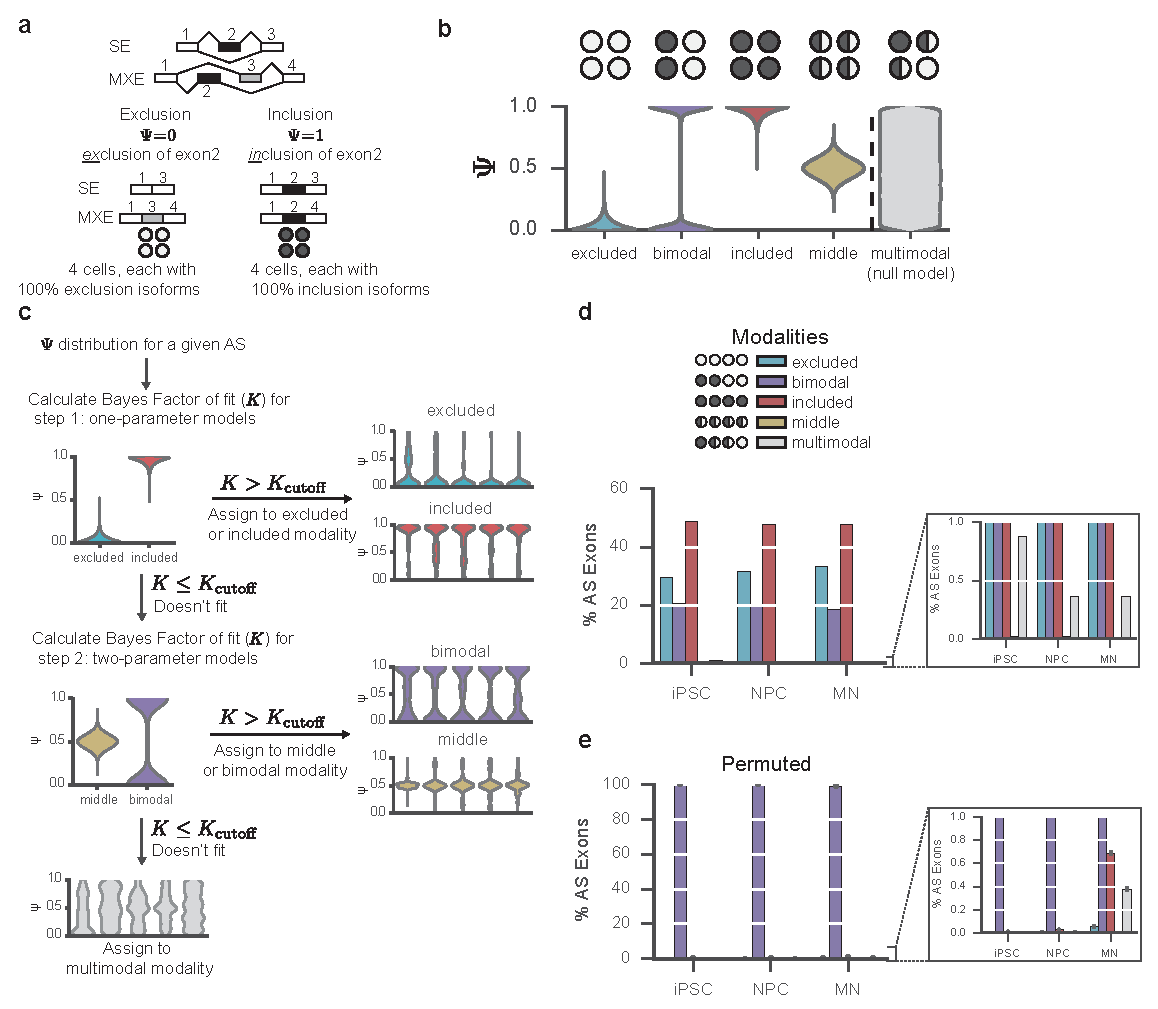
\includegraphics[width=5.8in]{figures/anchor_overview.pdf}
\end{figure}
%and, I'm not sure why, but one of the times I used this code the figure number wasn't augmented for the next figure, so check your figure numbers and if necessary uncomment the following line
%\addtocounter{figure}{1}
\clearpage
% --- END manual facingcaption for Figure 2 from paper --- %



% --- BEGIN manual facingcaption for Figure 3 from paper --- %
\clearpage
\thispagestyle{facingcaption}
\begin{figure}[h]
\captionsetup{labelformat=prev-page}
\caption[Bimodal AS events exhibit distinct sequence and evolutionary features.]{
Bimodal AS events exhibit distinct sequence and evolutionary features.\\
All results are shown for iPSCs that have highest number of AS events (12,690). Results are similar in three cell-types, except where indicated. All q-values of significance were derived from multiple hypothesis corrected (Bonferonni) non-parametric Mann-Whitney U test, unless otherwise indicated.\\
\textbf{a.}~Cumulative distributions of the mean Placental Mammal PhastCons score in each modality are shown, with constitutive exons as comparison. AS exons from included modality (red) are as conserved as constitutive exons (black), while excluded exons (blue) are least conserved, followed by bimodal (purple) and multimodal (grey) exons. right, heatmap of pairwise significance scores between each modality or constitutive exons (right panel).\\
\textbf{b.}~Mean Placental Mammal PhastCons scores of flanking intronic regions of exons in excluded (blue) bimodal (purple), multimodal (grey), included (red) modalities, and constitutive (black) exons in all cell-types. bottom, heatmap of base-wise significance of PhastCons scores is presented 0 <  for clarity.\\
\textbf{c.}~Phylostratum scores are summarized for genes harboring AS events in each modality together with genes containing constitutive exons. right, heatmap of pairwise significance scores between each modality or constitutive exons.\\
\textbf{d.}~Alternative splicing events conserved in mammals were extracted from Merkin et al, 2012 (Merkin et al., 2012) and their percentage among each modality is calculated. Hypergeometric test (multiple hypothesis corrected with Bonferonni) indicated q < 10-5 statistical significance. Fraction indicates No. of conserved events in each modality(nominator)/total events in the modality(denominator)\\
\textbf{e.}~Intron lengths summarized in excluded, bimodal, multimodal, included modality together with constitutive exons. top, heatmap of pairwise significance scores between each modality or constitutive exons.\\
\textbf{f.}~Conserved intronic sequences in each modality are enriched with distinct nucleotides. Motifs enriched for each modality are presented by PCA, shown with each circle as a motif and the vectors as component loadings of intron groups. left, Representative motifs are annotated with logos from the CISBP database. right, A simplified illustration of distinct nucleotide enrichment in each intron group. An interactive version of this plot is available at \url{https://plot.ly/~OlgaBotvinnik/32/cisbp-motif-t-test-enrichments-background-phenotype/}
}
\label{fig:modality_features}
\end{figure}
\clearpage
\begin{figure}[h]
\ContinuedFloat
\captionsetup{labelformat=empty}
\centering
% \includegraphics[width=5.8in]{sandiego.jpg}
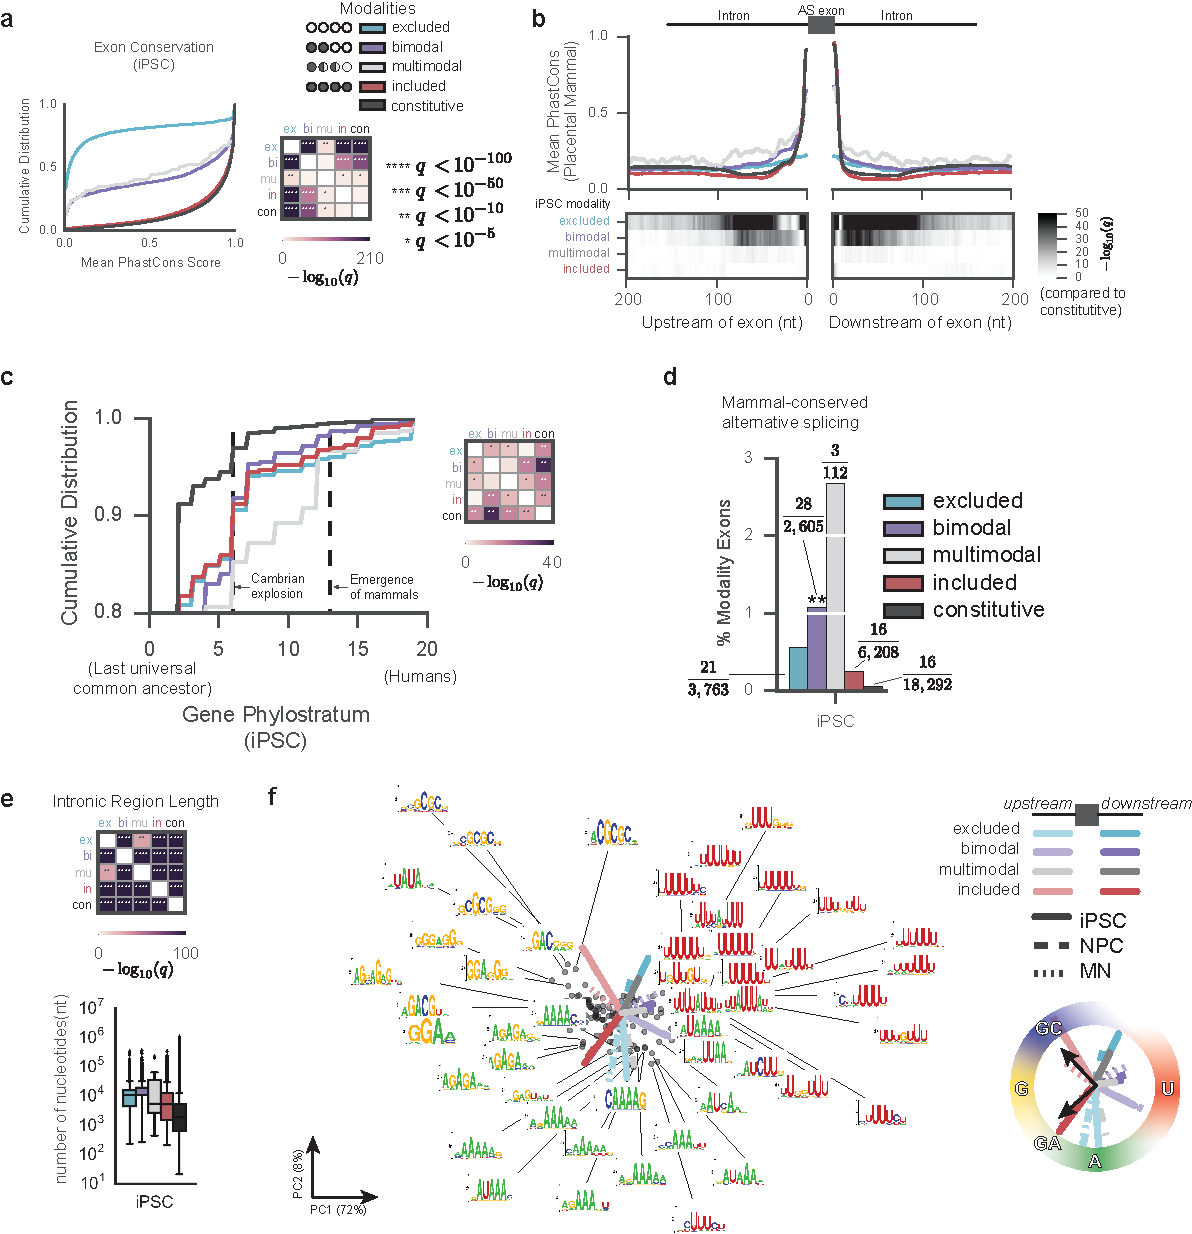
\includegraphics[width=5.8in]{figures/modality_features.pdf}
\end{figure}
%and, I'm not sure why, but one of the times I used this code the figure number wasn't augmented for the next figure, so check your figure numbers and if necessary uncomment the following line
%\addtocounter{figure}{1}
\clearpage
% --- END manual facingcaption for Figure 3 from paper --- %



% --- BEGIN manual facingcaption for Figure 4 from paper --- %
\clearpage
\thispagestyle{facingcaption}
\begin{figure}[h]
\captionsetup{labelformat=prev-page}
\caption[Dynamic AS events are primarily contributed by highly variant bimodal and multimodal events.]{Dynamic AS events are primarily contributed by highly variant bimodal and multimodal events.\\
\textbf{a.}~AS events change modalities during iPSC to MN transition. A total of 5,675 AS events was identified as common ones in both iPSCs and MNs. The compartmentalization of these common events in five modalities is presented in iPSCs (y-axis) against their corresponding modalities in MNs (x-axis). Gradient of heat map represents the percent of events in the iPSC modality row, annotated with the exact number of events. The diagonal indicates events remained in the same modality. Notably, 88\% of excluded events in iPSCs remained in excluded modality, and 86\% of included events in iPSCs remained as included in MNs. In contrast 52\% of bimodal events in iPSCs switch to either included or excluded modalities in MNs. Multiple hypothesis corrected (Bonferonni) hypergeometric tests were used to calculate significance.\\
\textbf{b.}~During the differentiation from iPSCs to MNs or from iPSCs to NPCs, we found 1,586 (17.6\%) or 1,029 (18.0\%) AS events switched modality, respectively.
\textbf{c.}~Within the switching events, 99\% events either switched from a bimodal/multimodal state or switched towards a bimodal/multimodal state. Around 1\% of switching events were observed among other types of modality changes.\\
\textbf{d-f.}~AS events in bimodal modality exhibits flexibility in protein coding.
\textbf{d.}~Schematic of predicted translation changes associated with AS exon inclusion.\\ Exclusion and inclusion of AS exon is termed as Isoform A and Isoform B, respectively. Six categories of coding outcomes are depicted when the isoform switch occurs. Pink, highlights creation of translated proteins or protein domain clades when AS exon is included. Purple, represents maintenance of protein clades with or without change of domain clades. Blue, represents loss of domain clades or disruption of translation when AS exon become included. The square and circle illustrate different Pfam domain clades. The square with dashed outline represents translated protein, possibly containing a Pfam domain clade.\\
\textbf{e.}~The coding outcomes are summarized in the six categories based on all AS events. The percentage of each translation configuration is used as the background distribution for significance calculations in \textbf{f}.\\
\textbf{f.}~AS events in bimodal modality favor protein and domain maintenance. The dominant isoforms in included and excluded modalities favor protein or domain creation and switching to the other isoform results in overwhelming disruption of protein coding. Enrichment is calculated against population average (shown in e) in each category using multiple hypothesis test corrected hypergeometric tests. *: $q< 10^{-10}$  **: $q< 10^{-100}$
}
\label{fig:dynamic_modalities}
\end{figure}
\clearpage
\begin{figure}[h]
\ContinuedFloat
\captionsetup{labelformat=empty}
\centering
% \includegraphics[width=5.8in]{sandiego.jpg}
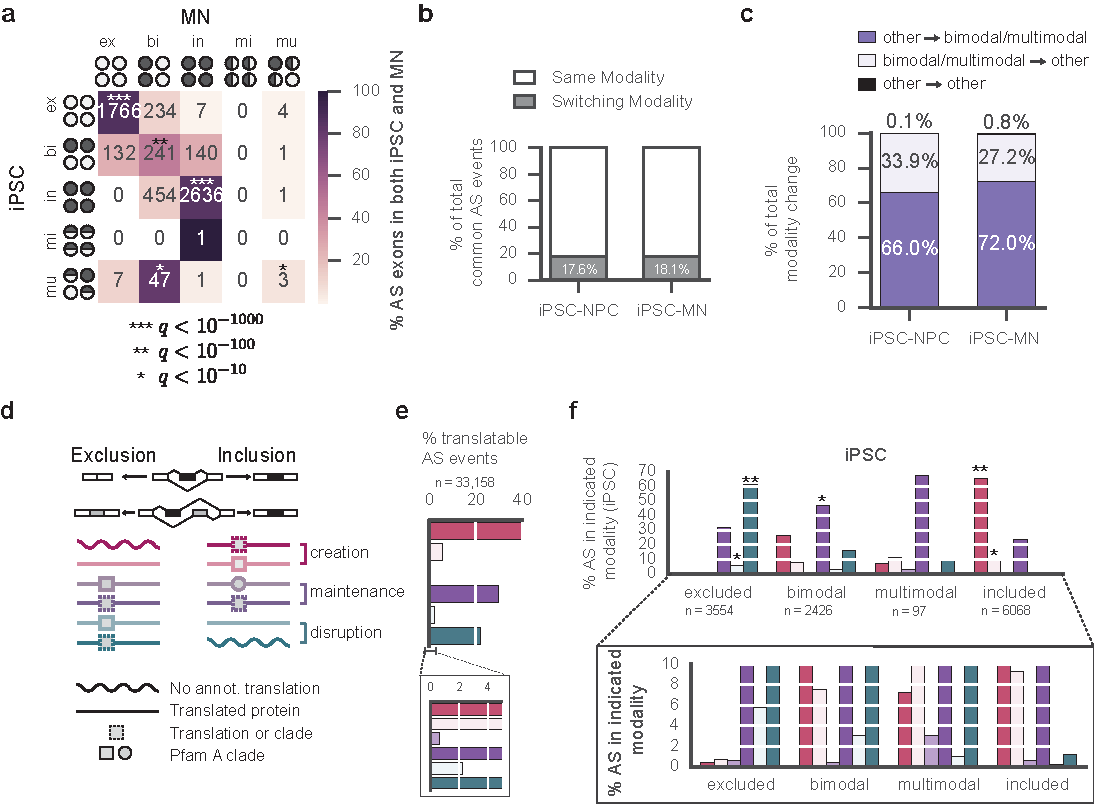
\includegraphics[width=5.8in]{figures/dynamic_modalities.pdf}
\end{figure}
%and, I'm not sure why, but one of the times I used this code the figure number wasn't augmented for the next figure, so check your figure numbers and if necessary uncomment the following line
%\addtocounter{figure}{1}
\clearpage
% --- END manual facingcaption for Figure 4 from paper --- %


% --- BEGIN manual facingcaption for Figure 5 from paper --- %
\clearpage
\thispagestyle{facingcaption}
\begin{figure}[h]
\captionsetup{labelformat=prev-page}
\caption[Bimodal and multimodal AS events reveal subpopulations invisible by gene expression alone.]{Bimodal and multimodal AS events reveal subpopulations invisible by gene expression alone.\\
\textbf{a-g.} SNAP25 alternative splicing reveals a more mature subpopulation in motor neuron population.\\
\textbf{a.}~SNAP25 is primarily expressed in MNs. \\
\textbf{b.}~Usage of alternative exon 5 (a MXE containing exon 5a and exon 5b) in the three populations. Shown is the usage of alternative exon 5a of SNAP25. \\
\textbf{c.}~Summary of exon 5 usage in motor neurons.\\
\textbf{d.}~Preferential usage of exon 5a or exon 5b of SNAP25 in MNs reveals intricate cell states. Genes correlated with the Psi score of this MXE in SNAP25 (above an empirical threshold) were used to cluster all MNs containing this event. Two main subgroups are observed, one with Psi close to 1 (red in the legend bar), the other with Psi close to 0 (blue in the legend bar). Cells with Psi around 0.5 are illustrated with yellow. Black and light grey indicate qualified and outlier MNs based on $k$-means clustering, respectively. Gradient of purple indicates gene expression in $\log_2(\text{TPM}+1)$, with darker being highly expressed. A few representative genes from the two subgroups are highlighted. \\
\textbf{e.}~Examples of representative genes correlating with Psi of this MXE in SNAP25. KATNAL1 and ANAPC16 are more enriched in the cells with $\Psi \approx 1$. DCTN1 and PCLO are more enriched in the cells with $\Psi \approx 0$. X-axis represents the Psi score, and y-axis represent gene expression in $\log_2(\text{TPM}+1)$. Each MN is depicted as a green circle. Solid green line represents simple linear regression line between Psi and the expression of indicated genes. Shaded green represents 95\% confidence interval of the regression.\\
\textbf{f-g.}~Genes correlating with this MXE event distinguish the two subgroups of MNs. Each MN is depicted as a dot in PCA.  Red: cells with $\Psi \approx 1$; blue: $\Psi \approx 0$; yellow: $\Psi \approx 0.5$; X: cells with a Psi assigned as NA.\\
\textbf{f.}~PCA of all expressed genes in MNs failed to separate the two subgroups.\\
\textbf{g.}~Using only the genes correlated with Psi of the MXE in SNAP25, two subgroups are readily separated. Percentage of variance explained are labeled at each PC.\\
\textbf{h-m.}~A bimodal SE event in DYNC1I2 as an example to dissect NPCs into a more proliferating subgroup and a subgroup on the trajectory of neuronal differentiation.\\
\textbf{h.}~Expression of DYNC1I2 in the three populations.\\
\textbf{i.}~Psi distribution of a SE event in DYNC1I2 in the three populations. This event is bimodal in both iPSCs, NPCs and becomes included in MNs.\\
\textbf{j.}~Genes correlating with Psi of this SE event is able to cluster the NPCs into two subgroups. Rows represent the genes and columns represent single cells in NPCs. Genes detected in NPC and correlated with Psi (Spearman $R > 0.5$). Green: NPC. Blue: cells with Psi around 0. Red: cells with Psi around 1. Light Blue to yellow: cells with Psi around 0.5. Black and grey: cells designated as qualified cells versus outlier-cells based on k-means clustering. Representative genes enriched in the two subgroups are highlighted in blue or red. \\
\textbf{k.}~Example genes enriched in the two subgroups of NPCs. ONECUT2 and DCC are more highly expressed in cells with $\Psi \approx 1$; ORC3 and MKI67 are more highly expressed in cells with $\Psi \approx 0$. Psi scores of the SE in DYNC1I2 is plot on x-axis and expression of indicated genes is plotted on y-axis.\\
\textbf{l-m.}~Only genes correlating with Psi are able to separate two subgroups in NPCs, with each NPC depicted as a dot in the PCA. Red: cells with $\Psi \approx 1$; blue: $\Psi \approx 0$; yellow: $\Psi \approx 0.5$; X: cells with a Psi assigned as NA. \\
\textbf{l}.~PCA of all expressed genes in NPCs failed to separate the two subgroups.\\
\textbf{m.}~Genes correlating with Psi are able to segregate the two subgroups by PCA.
}
\label{fig:hidden_cell_states}
\end{figure}
\clearpage
\begin{figure}[h]
\ContinuedFloat
\captionsetup{labelformat=empty}
\centering
% \includegraphics[width=5.8in]{sandiego.jpg}
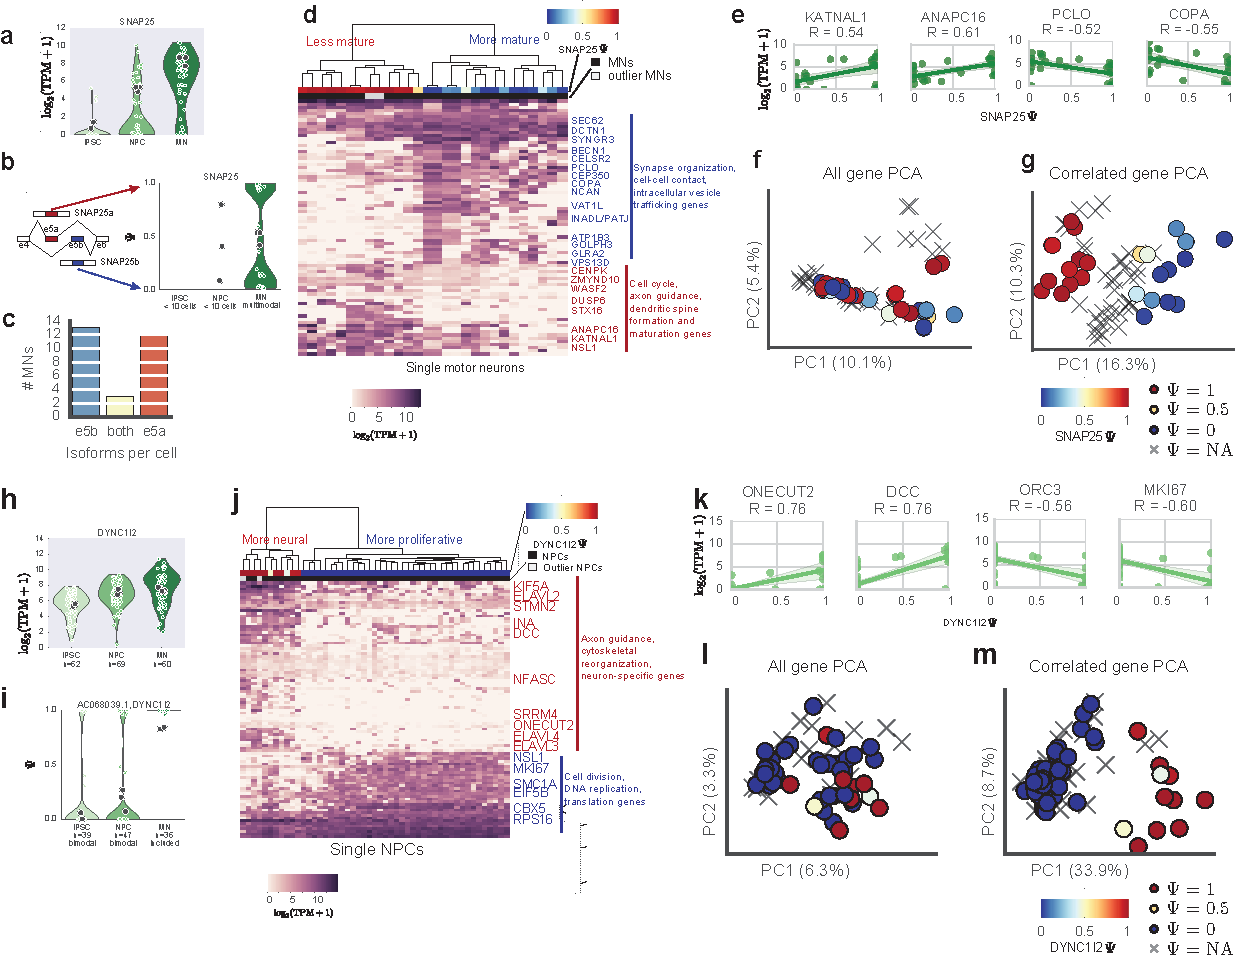
\includegraphics[width=5.8in]{figures/hidden_cell_states.pdf}
\end{figure}
%and, I'm not sure why, but one of the times I used this code the figure number wasn't augmented for the next figure, so check your figure numbers and if necessary uncomment the following line
%\addtocounter{figure}{1}
\clearpage
% --- END manual facingcaption for Figure 5 from paper --- %


% --- BEGIN manual facingcaption for Figure 6 from paper --- %
\clearpage
\thispagestyle{facingcaption}
\begin{figure}[h]
\captionsetup{labelformat=prev-page}
\caption[Bonvoyage visualizes dynamic AS changes.]{Bonvoyage visualizes dynamic AS changes.\\
\textbf{a.}~A schematic to illustrate the transformation of splicing profiles into the two-dimensional waypoint space by bonvoyage. Splicing distribution of each event (A, B, C and D represent 4 different AS events) was discretized into bins (left), factorized by non-negative matrix factorization (NMF) and projected onto 2-dimensional space (middle), such that each data point represents a distribution of alternative splicing. The origin point represents a distribution that all cells have 50\% of inclusion and 50\% exclusion reads observed in scRNA-seq. When the distributions of the same event (either event B or C) are visualized in two different cell-types or states, the dynamic of the event is illustrated by its voyage in the waypoint space (right panel).\\
\textbf{b.}~AS events in iPSCs projected in the waypoint space. The shade of hexagon indicates the number of events. \\
\textbf{c.}~AS events in iPSCs (same as \textbf{b}), colored by the modality estimated by anchor. Each dot represents distribution of one AS event. Note, each modality occupies a distinct region of the waypoint space. Black-outlined circle highlights PKM MXE event.\\
\textbf{d.}~AS events in MNs are colored by their modalities and presented in waypoint space. Black-outlined square highlights PKM MXE event.\\
\textbf{e.}~Dynamics of the MXE event in PKM is illustrated in the waypoint space. Shown is the inclusion of exon 9 of the MXE, which is included in both iPSCs and NPCs and becomes bimodal in MNs.\\
\textbf{f-g.}~Global splicing dynamics between iPSC and MN, aggregated by voyage direction instead of modalities. \\
\textbf{f.}~Number of events originated in iPSC and travel in the indicated directions to land in excluded, bimodal, included, middle, or multimodal modality in MN. \\
\textbf{g.}~Same data as (\textbf{f}), visualized by vectors representing the iPSC (tail) and MN (tip) position of the alternative exon. Color of arrows are coded based on event modalities in iPSCs.
}
\label{fig:bonvoyage_overview}
\end{figure}
\clearpage
\begin{figure}[h]
\ContinuedFloat
\captionsetup{labelformat=empty}
\centering
% \includegraphics[width=5.8in]{sandiego.jpg}
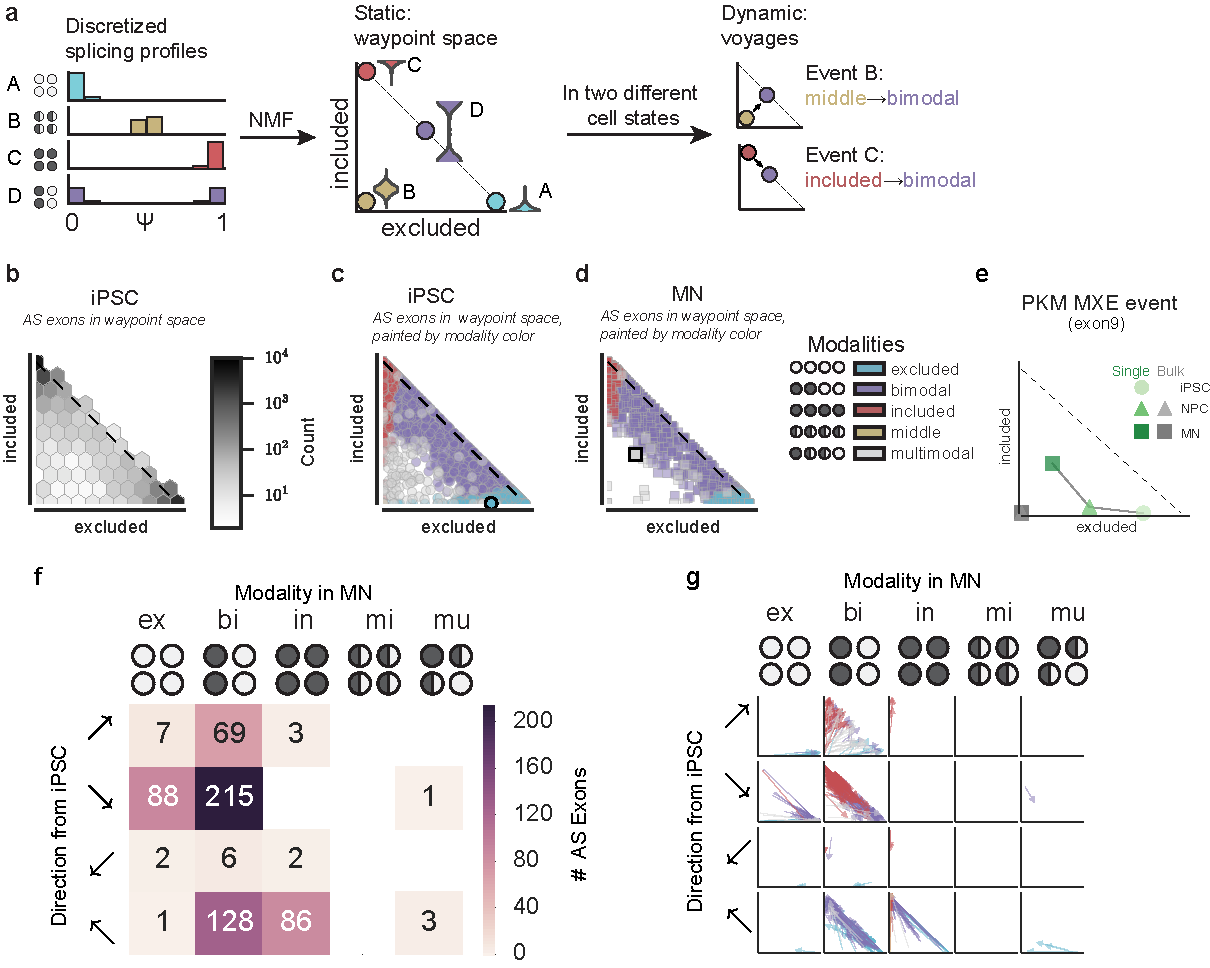
\includegraphics[width=5.8in]{figures/bonvoyage_overview.pdf}
\end{figure}
%and, I'm not sure why, but one of the times I used this code the figure number wasn't augmented for the next figure, so check your figure numbers and if necessary uncomment the following line
%\addtocounter{figure}{1}
\clearpage
% --- END manual facingcaption for Figure 6 from paper --- %

% --- BEGIN manual facingcaption for Figure 7 from paper --- %
\clearpage
\thispagestyle{facingcaption}
\begin{figure}[h]
\captionsetup{labelformat=prev-page}
\caption[qPCR validation and summary of biological findings.]{qPCR validation and summary of biological findings.\\
\textbf{a-b.}~Waypoint-weighted protein properties changing between iPSC and MN. Significant changes(blue) are identified by a factor of three on Mahalanobis distance relative to all iPSC-MN comparisons.\\
\textbf{a.}~Protein disorder by IUPred, where a score above 0.5 (red dashed line) indicates disorder.\\
\textbf{b.}~Isoelectric point (pI), where the black dashed line indicates $\text{pI}=7$. X-axis, weighted protein property in iPSC and y-axis, weighted protein property in MN.
\textbf{c-f.}~Distribution of AS inclusion is verified by single cell qRT-PCR (sc-qPCR). Primer sets for inclusion, exclusion and gene expression were designed for each event tested. Percent inclusion measured in sc-qPCR is calculated by $\frac{2^{\text{inclusion Ct}}}{2^{\text{inclusion Ct}} + 2^{\text{exclusion Ct}}}$ (See Methods for more details) in both iPSCs ($n =134$) and MNs ($n = 95$). \\
\textbf{c.}~Percent spliced-in (Psi/$\Psi$) distributions for RPS24 exon 5 measured by single-cell RNA-Seq shown as violinplots (left) and voyages (right).\\
\textbf{d.}~Percent exon inclusion distributions for RPS24 exon 5 measured by single-cell qPCR shown as violinplots (left) and voyages (right).\\
\textbf{e.}~Percent spliced-in (Psi/$\Psi$) distributions for ZNF207 exon 9 measured by single-cell RNA-seq shown as violinplots (left) and voyages (right).\\
\textbf{f.}~Percent exon inclusion distributions for ZNF207 exon 9 measured by single-cell qPCR shown as violinplots (left) and voyages (right).\\
\textbf{g.}~Summary: At single cell resolution, three main categories of modalities can be identified: included, excluded and bimodal. Each modality has unique sequence, coding and evolutionary features. During cell differentiation, majority of unimodal events are static, whereas the highly variance events are dynamic, playing a key role in shaping the transcriptome.
}
\label{fig:validation_summary}
\end{figure}
\clearpage
\begin{figure}[h]
\ContinuedFloat
\captionsetup{labelformat=empty}
\centering
% \includegraphics[width=5.8in]{sandiego.jpg}
\includegraphics[width=5.8in]{figures/validation_summary.pdf}
\end{figure}
%and, I'm not sure why, but one of the times I used this code the figure number wasn't augmented for the next figure, so check your figure numbers and if necessary uncomment the following line
%\addtocounter{figure}{1}
\clearpage
% --- END manual facingcaption for Figure 7 from paper --- %



\begin{figure}[h]
  \centering
  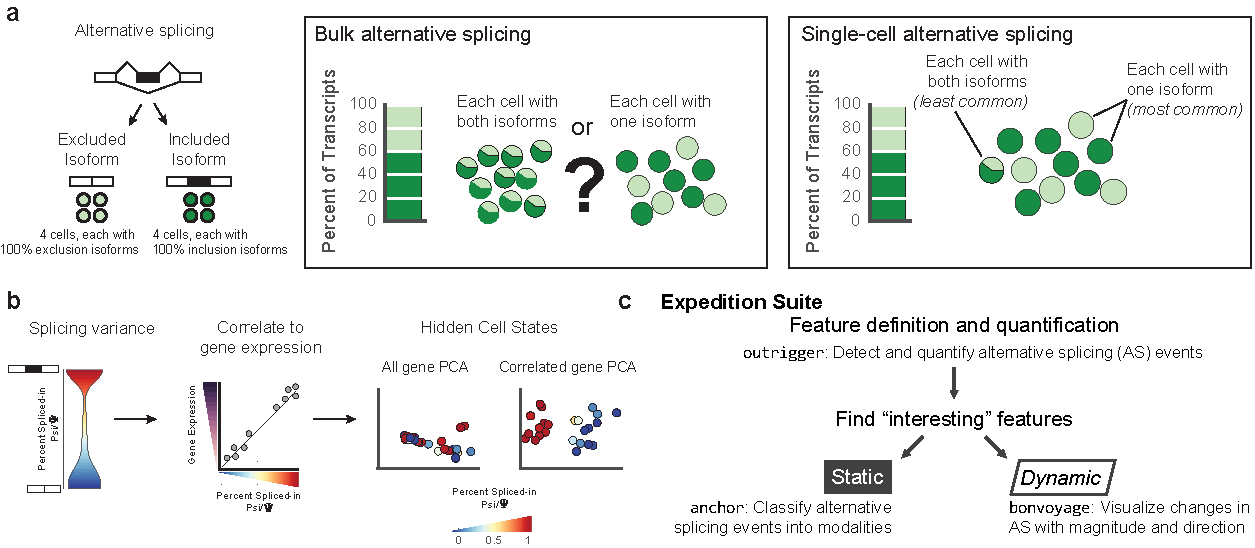
\includegraphics[width=5.8in]{figures/graphical_abstract.pdf}
  \caption{Graphical abstract of findings.}
  \label{fig:graphical_abstract}
\end{figure}

\section{Methods}

% For some reason have to add the paragraph indent size here because
% it gets ignored if it's only in the preamble
% \setlength\parindent{24pt}


\subsection{Cell culture and differentiation}

iPSCs were cultured on matrigel coated plated using mTeSR (Stem Cell Technologies) media with mTeSR supplement at $37^\circ$ C incubator with 5\% CO$_{2}$.\par

Neuronal progenitor cells (NPCs) were differentiated from iPSCs. Briefly, iPSCs were cultured in Matrigel coated plates and dislodged by dispase. To form embryonic bodies, the dislodged colonies were cultured in DMEM/F12 (Invitrogen) with GlutaMax and N2 supplement in non-adhere petri dish. Media were replaced every other day for 7 days. EBs were then plated onto matrigel coated plate to allow rosette formation. Clean rosette were picked manually and maintained in EB media for 7 days and subsequently dissociated with accutase and cultured in NPC media (DMEM/F12, GlutaMax, N2 and B27 with \SI[per-mode=symbol]{2}{\micro\gram\per\micro\liter} FGF) to allow neuron progenitor cell differentiation. NPCs were maintained in NPC media.

Motor neurons were directly differentiated from iPSCs as previous described\cite{Chambers:2009ey}. Briefly, iPSCs were cultured on matrigel coated plates until fully confluent in mTeSR then switch to knock-out serum replacement media (KSR) containing Dorsomorphin(\SI{1}{\micro\Molar}) and SB431542 (\SI{10}{\micro\Molar}). Upon day 4 of differentiation, increasing amounts of N2 media (25\%, 50\%) was added to the KSR. From day 7 of differentiation, \SI{1.5}{\micro\Molar} retinoic acid and \SI{200}{\nano\Molar} Smoothened Agonist (SAG, EMD Millipore) were added to induce patterning. Cells were dissociated on day 17 of differentiation and replated in poly-D-lysine and laminin coated plates. Maturation was performed using BDGF (\SI[per-mode=symbol]{2}{\nano\gram\per\micro\liter}), GDNF (\SI[per-mode=symbol]{2}{\nano\gram\per\micro\liter}), CNTF (\SI[per-mode=symbol]{2}{\nano\gram\per\micro\liter}), ascorbid acid, sonic hedgehog and retinoic acid in N2 and B27 media up until 35 days of differentiation.


\subsection{Single-cell capture and library preparation}

iPSCs, NPCs and MNs were dissociated using Accutase (Stem Cell\\Biotechnologies) and filtered through \SI{40}{\micro\meter} cell strainers to obtain single cell suspension. Single cells were captured on C1 auto prep platform (Fluidigm, CA) according to manufacturer's instructions. C1 auto prep chips were visually inspected with a light microscopy at 20X to ensure singularity of captured cells. All non-single cells were discarded from analysis. SMARTer Ultra Low RNA cDNA Synthesis Kit (Clontech) was used to reverse transcribe polyA-tailed RNA. cDNA was amplified using Advantage 2 Polymerase Mix by PCR at \SI{95}{\degreeCelsius} for 1 minutes, followed by 21 cycles of 15 seconds at \SI{95}{\degreeCelsius}, 30 seconds at \SI{65}{\degreeCelsius} and 6 minutes at \SI{68}{\degreeCelsius}, followed by another 10 minutes at \SI{72}{\degreeCelsius} as a final extension. cDNAs were inspected using Agilent Bioanalyzer High Sensitivity DNA chips and quantitated by PicoGreen dsDNA Assay kit (ThermoFisher). cDNAs were diluted to \SI{1}{\nano\gram} to generate libraries using the Nextera XT DNA kit (Illumina, La Jolla, CA). Libraries were multiplexed and sequenced on Illumina HiSeq 2000 to generate 100bp PE reads.

\subsection{RNA-Seq processing}

RNA-seq reads were trimmed using \texttt{cutadapt} v1.8.1 of adapter sequences \texttt{TCGTATGCCGTCTTCTGCTTG}, \texttt{ATCTCGTATGCCGTCTTCTGCTTG}, \\\texttt{CGACAGGTTCAGAGTTCTACAGTCCGACGATC}, \texttt{GATCGGAAGAGCACACGTCTGAACTCCAGTCAC}, $\left[\text{\texttt{A}}\right]_{50}$, $\left[\text{\texttt{T}}\right]_{50}$, mapped to repetitive elements (RepBase v18.05 \cite{Jurka:2005tp}) using the STAR\cite{Dobin:2013fg} splicing-aware aligner (v2.4.01). Reads that did not map to repetitive elements were then mapped to the human genome (hg19), using GENCODE\cite{Harrow:2012cx} (v19) gene annotations to create the splice junction database. We used the  \texttt{SJ.out.tab} files from STAR to create alternative splicing annotations and calcluate percent spliced-in (see Sec.~\ref{sec:outrigger}). Gene expression was quantified with sailfish\cite{Patro:2014jd} using GENCODE v19 protein-coding and long non-coding RNA annotation, and we then aggregated transcript-level expression to genes.

% \subsection{PCR duplicate removal}

% We removed reads which had exactly the same sequence and alignment location using the command \texttt{rmdup} from the \texttt{samtools} suite\cite{Li:2009kaa}. We then indexed the duplicate-removed .bam files with \texttt{samtools index}.

\subsection{Single-cell expression-level quality control and outlier detection}

We retained genes expressed with TPM $> 1$ in at least 10 cells for a total of 18,594 genes, and filtered out cells which had $<4,000$ expressed genes, which was a natural cutoff in the data. For the three cell types, $n=63$ iPSCs, $n=73$ NPCs, and $n=70$ MNs had enough expressed genes to pass gene expression level quality control.

% \subsection{Outlier detection}

We performed $K$-means clustering with $k=3$ on the gene expression matrix, with 1000 different random initializations. For each cell that clustered into a group that consisted of a majority of a different cell type (e.g. a motor neuron that was clustered in the group with majority NPCs), we called these cells outliers and discarded them from analysis. Overall, for iPSC: 71 were captured, 63 passed  QC,  1 outlier for 62 total; for NPC: $98$ were captured, 73 passed QC, 4 outliers for 69 total; for MN: $93$ were captured,  70 passed QC, 10 outliers for 60 total.

% iPSC: 71 were captured, 64 passed  QC,  1 outlier for 63 total; for NPC: 65 + 33 CVN = 98 captured, 76 passed QC, 3 outliers for 73 total; for MN: 63 + 30 = 93 captured,  79 passed QC, 9 outliers for 70 total.


\subsection{Estimation of alternative splicing}
We used \outrigger\, to create a custom alternative splicing index on the splice junction (\texttt{SJ.out.tab}) files created by STAR, and used GENCODE v19 to define possible exons. This created $40,534$ skipped exon (SE) and $13,217$ mutually exclusive exon (MXE) possible alternative events, and we calculated percent spliced-in (Psi/$\Psi$) with a minimum of 10 junction reads. We then filtered for events that were alternative, not constitutively included or excluded across all cells. Alternative events were defined by, $0 < \Psi < 1$, $\Psi \neq 0, 1$ in at least one cell. Events were then filtered for events that were detected in at least 10 cells of any celltype, resulting in $13,910$ events.

% \subsection{Quality control of AS using split single cell libraries}
% To ensure that variations in alternative splicing detection is not due to technical variation in our experimental procedure, we assessed robustness in estimating AS events from single cells by comparing AS events from paired libraries generated from divided single-cells (\textbf{Supplementary Fig.~\ref{fig:splicing_qc}c}). We observed that 60\% of the $15,000$-$18,000$ estimated AS events from the ``splits'' of each cell overlap, with a statistically significant correlation in the percent-spliced-in (Psi/$\Psi$) values (Spearman correlation $R~1$; $p$-value $~0$, \textbf{Supplementary Fig.~\ref{fig:splicing_qc}d}, top row) for the shared AS events. In contrast, when two libraries from distinct single IPS cells were compared, the correlation was high but lower than for the split cells (Spearman correlation $R=0.9$, $p~0$; \textbf{Supplementary Fig.~\ref{fig:splicing_qc}d}, bottom row). Furthermore, the pooled samples' expression and splicing was highly correlated (Spearman $R=0.94$ and $R=0.97$, respectively; \textbf{Supplementary Fig.~\ref{fig:splicing_qc}e}, bottom row), but compared to a split cell, the expression and splicing correlations were smaller (Spearman $R=0.71$ and $R=0.932$, respectively; \textbf{Supplementary Fig.~\ref{fig:splicing_qc}e}, top row).

\subsection{Constitutive exons}

We defined constitutive exons as those that did not appear as the alternative exon in any of the splice types (MXE and SE), and had at least 10 reads on both upstream and downstream junctions, in at leat 10 cells per cell type.

\subsection{ICA on constitutively expressed genes and their splicing events}
First, $12,685$ genes were identified as non-DE genes across the three populations using a non-parametric Kruskal-Wallis test with Bonferroni-corrected $p$-value, called $q$, with $q > 10$ as the cutoff.

Second, AS events were extracted from non-DE genes and their Psi scores are subjected to Independent Component Analysis (ICA). To impute the null values widespread in splicing data, we replaced NAs with an arbitrary number (100) out the of range of Psi values. We did not find that the choice of the arbitrary number affected the ICA results. We then calculated ICA on the imputed matrix.

\subsection{Hierarchical clustering}

We performed hierarchical clustering on samples in Python, using the \texttt{fastcluster}\cite{Mullner:2013bl} package and performing optimal leaf ordering\cite{BarJoseph:2001tr} using the \texttt{polo}\cite{Anonymous:2FB4UNR9} package. All clustering was performed using the Euclidean distance metric with Ward's method\cite{WardJr:2012te}. We visualized using the matplotlib\cite{Anonymous:matplotlib} and seaborn\cite{Anonymous:hWlQiCz3} visualization libraries in Python.

\subsection{Gene Ontology Enrichment}
We calculated Gene Ontology (GO) enrichment by using the Gene Ontology mapping queried to the Entrez gene database using the Python package \texttt{mygene}\cite{Wu:2012bo,Xin:2016fv}. We calculated GO enrichment using only the ``biological process'' category, and corrected for multiple hypothesis testing using Bonferroni correction as performed in the Python package \texttt{goatools}\cite{Tang:2015ub}.

\subsection{Categorization of alternative splicing ``modes''}
We calculated modality using the default parameters of the \anchor\, software (see Sec.~\ref{sec:anchor}) only on splicing events observed in at least 10 cells per cell-type. The performance of anchor was tested extensively using simulated data in comparison to existing bimodality detecting methods.

\subsection{Sequence annotation of alternative isoforms}

We annotated alternative events and their biological features at different levels of the Central Dogma.

\subsubsection{DNA-level}

\paragraph{Evolutionary conservation.} We used units of evolutionary conservation as measured by Placental Mammal PhastCons\cite{Siepel:2005cu} scores calculated previously\cite{Lovci:2013cq} (\textbf{Figure~3a-b}, \textbf{Supplementary Fig.~\ref{fig:modality_features}}).

For average conservation of exons, we used \texttt{bigWigAverageOverBed}\cite{Kent:2010ff} to calculate the mean conservation (treating bases without annotated conservation as NA) across each exon. For base-wise conservation, we used the HTSeq\cite{Anders:2015gf} Python package to create a memory-mapped \texttt{GenomicArray}, and queried this object with the intronic intervals.


\paragraph{Repetitive element overlap.} We used the Repeat Masker track\cite{Rosenbloom:2015bg} from UCSC's Genome Browser\cite{Kent:2002bwa} and used \texttt{bedtools intersect}\cite{Quinlan:2010kma} to overlap with our exon definitions. We grouped repeats into families defined by the Dfam\cite{Hubley:2016fu} database of repetitive DNA elements (\textbf{Supplementary Fig.~\ref{fig:modality_features}e}). For simplicity of interpretation, we used only repetitive elements that appeared at least 10 times in the excluded modality, as it was the modality with the most repetitive elements.

\paragraph{Gene age (Phylostratum)}

We used the Phylostratum classification of genes as found previously\cite{DomazetLoso:2008ba} (\textbf{Figure~3e}). For each splicing event, we found all overlapping genes in the same genomic locus, and aggregated all genes with at least one event in each modality. Meaning, a gene could appear in multiple modality categories if it had one exon in the included modality and another in the bimodal category.


\paragraph{$k$-mer counting and motif (PWM) enrichment}
We used placental mammal conserved elements as downloaded from UCSC\cite{Rosenbloom:2015bg}, taking only conserved elements upstream and downstream of alternative exons. We used \texttt{kvector}\cite{Anonymous:ug} to count $k$-mers in these conserved elements, and calculated a $Z$-score of $k$-mer enrichment for each intron group defined by cell-type, intron context, and modality (\textbf{Supplementary Fig.~\ref{fig:modality_features}k-l}, \textbf{Figure~3d}). Interested in which $k$-mers were enriched in each modality, we used the total $k$-mer counts in the intron context and celltype, for all modalities, as the background. We then performed principal component analysis using the Python package \texttt{scikit-learn}\cite{Pedregosa:2011tv} on the modality introns (\textbf{Supplementary Fig.~\ref{fig:modality_features}m}). We labeled $k$-mers by the standard color of the majority nucleotide (if there was a tie for the winner, the $k$-mer was assigned grey) whose squared PCA distance was greater than two squared standard deviations from the center, i.e. an ellipse around the origin of the plot. We used the Python package \texttt{adjustText}\cite{Anonymous:tk} to move the text labels away from each other and make them readable.

To find which RNA binding protein motifs were enriched for different modalities, we used version 0.6 of the CISBP-RNA binding database\cite{Ray:2013br} and transformed each position-weight matrix (PWM) into a Boolean vector of $k$-mers that could exactly fit into the PWM, with no mis-matches (\textbf{Supplementary Fig.~\ref{fig:modality_features}n-o}). We ignored psuedocounts by setting all values $\leq 0.1$ to zero. We then used this Boolean matrix to obtain motif $k$-mers and calcluate enrichment using a $t$-test, as compared to all $k$-mers of that intron group. We then performed PCA on the motif $t$-statistics, using the intron groups as features (\textbf{Supplementary Fig.~\ref{fig:modality_features}p}, \textbf{Figure~3d}). We labeled motifs whose squared PCA distance was greater than two squared standard deviations from the center, i.e. an ellipse around the origin of the plot. We used the Python package \texttt{adjustText}\cite{Anonymous:tk} to move the text labels away from each other and make them readable.


\subsubsection{RNA-level}

\paragraph{Consistency of splicing between bulk and single-cells}
To calculate the total difference between the bulk $\Psi$ and single-cell $\Psi$ estimates, for each event, we calculated the average difference between the pooled sample $\Psi$ and every single-cell $\Psi$, much like a sample mean calculation (\textbf{Supplementary Fig.~\ref{fig:modality_features}a}).

\paragraph{Splice site strength}
We used \texttt{bedtools}\cite{Quinlan:2010kma} and \texttt{pybedtools}\cite{Dale:2011cl} to obtain the $5^\prime$ (relative to exon-intron boundary: -20nt into intron and +3nt into exon) and $3^\prime$ (relative to exon-intron boundary: -3 into exon and +6 into intron), and obtained the transcript sequences for these regions. We used MaxEntScan\cite{Yeo:2004fg} to calculate the strength of the alternative exon (exon 2 in both the SE and MXE cases) splice sites (\textbf{Supplementary Fig.~\ref{fig:modality_features}f-g}).

\paragraph{Expression of splicing events}
For finding the gene expression per splicing event, for each event, we used all genes that could map to it. Sometimes multiple genes could map to a single event, as a result of poor annotation, or multiple read-through transcripts. To mitigate this, for each event, we summed all gene expression by the $\log_2(\mathrm{TPM}+1)$ values, and plotted the distribution of expression per modality (\textbf{Supplementary Fig.~\ref{fig:modality_features}h}).

\paragraph{Intron and exon length}
As we used \outrigger\, to calculate splicing, it also output the lengths of the introns and exons for each alternative event, which is what we used (\textbf{Figure~3c} and \textbf{Supplementary Fig.~\ref{fig:modality_features}d}).


\subsubsection{Protein-level}

We are in the process of packaging the splicing event isoform translation and domain scanning code into a package called \texttt{poshsplice}\cite{Anonymous:uj}.

\paragraph{Protein translation}
Using events which had at least one isoform annotated with a CDS in GENCODE v19 ($22,152$ SE and MXE events), we translated the exon trio and duo (SE, included isoform has three exons and and excluded has two) or exon trios (MXE, both included and excluded isoforms contain three exons) to its transcript-annotated reading frame. If these exons participated in transcripts with multiple reading frames, we used all translations.

\paragraph{Domain search} We used the \texttt{hmmscan} command from the HMMer\cite{Finn:2011eg,Eddy:1998ut} software suite (v3.1b1) to search for protein domains matching those in the manually curated Pfam-A database\cite{Finn:2016bf}. We used a domain-independent E-value cutoff of $10^{-5}$. With this raw data, we observed ``domain switching'' between isoforms in instances such as ``Kinase'' to ``Tyrosine Kinase'', when indeed the exact characters of domain name changed, but the overall function didn't. To alleviate this problem, we aggregated domains into clades using Pfam's annotations. We then annotated each individual event with whether only the exclusion or inclusion isoforms had an annotated translation, only one isoform, contained a clade, both contained the same clade, or the clades switched (\textbf{Figure~4d}).

\subsection{Correlation of splicing to expression}
We correlated bimodal and multimodal splicing events to genes with variant expression, defined as two standard deviations away from the mean variance of all genes. We used Spearman correlation to compare splicing profiles to gene expression, and used a threshold of absolute correlation values $|R| > 0.5$ across all samples.

\subsection{Transformation of splicing profiles to 2d space}

We used \bonvoyage\, (see Sec.~\ref{sec:bonvoyage}) to transform one-dimensional splicing profiles into two-dimensional space (\textbf{Figure~6a-c}), using the default parameters. We performed the transformation within cell-type, and required at least 10 cells per splicing event to transform.

\subsection{Waypoint-weighted protein properties}

To obtain protein properties, we used IUPRED\cite{Dosztanyi:2005gq} to calculate protein disorder and the \texttt{ProtParam} module in BioPython\cite{Cock:2009hj} to calculate aromaticity, instability index, molecular weight, secondary structure properties (alpha-helix, beta-sheet, and turns), flexibility, grand average of hydropathy (GRAVY) and isoelectric point.



We summarized isoform protein properties for each phenotype by using the NMF-transformed waypoint space into a weighted average. Using $p_{\text{included}}$ and $p_{\text{excluded}}$ to represent the protein property value (e.g. molecular weight or disordered protein score) of each isoform, and $w_{\text{included}}$ and $w_{\text{excluded}}$ to represent the splicing event's waypoint space position for the included ($y$) and excluded ($x$) axes. We calculated the weighted protein property, $p_w$, within each phenotype, as we did for the modality and waypoint calculation.

\begin{align}
p_w = p_{\text{included}} w_{\text{included}} + p_{\text{excluded}} w_{\text{excluded}}
\end{align}

For properties that had a relative center, e.g. isolectric point which has a neutral value of 7, we subtracted the center value for each protein property, $p_{\text{center}}$ so the multiplication by the waypoint space would amplify the distance from center.

\begin{align}
p_w = p_{\text{center}} + (p_{\text{included}} - p_{\text{center}}) w_{\text{included}} + (p_{\text{excluded}} - p_{\text{center}}) w_{\text{excluded}}
\end{align}

\subsubsection{Voyaging protein properties}

Interested in which protein properties which changed significantly between cell types, we used Mahalonobis distance\cite{DeMaesschalck:2000hv} ($d_m$), a non-parametric method of finding outliers from distributions. In the two-dimensional case, this means values that are significantly ``off-diagonal'' when comparing two cell types, e.g. iPSC to MN. We used a multiplier of $3d_m$ as the threshold for highly changing protein properties.

\subsection{Single-cell qPCR and primer design}

Single iPSCs and differentiated MNs were captured on C1 auto prep platform (Fluidigm, CA). All non-single cells were discarded from analysis. cDNA from single cells were prepared using the Single-Cell-to-Ct kit (ThermoFisher, USA) and pre-amplified with a pool of primers designed for the splicing events and the expression of corresponding genes. Inclusion and exclusion primers were specifically designed to quantitate inclusion and exclusion of AS exons and expression primers were designed from constitutive exons. All primers were tested for amplification efficiency. High-throughout quantitative PCR was performed on 96.96 Dynamic Arrays on BioMark system (Fluidigm) according to manufacturer's instructions. Each pre-amplified STA sample was diluted 1:15 for iPSCs and 1:10 for MNs. 3 housekeeping genes (RPL22, RPL27, PGK) and lineage genes (POU5F1, LIN28A, DPPA2, ISL1, MNX1, STMN2, NFEL, DCX) were included. The full list of primers is available in \textbf{Supplementary Table 1}.

\subsection{qPCR data processing}

The log expression of each primer set $g$ was computed as $\log(E_{g,c}) = 25 - \mathrm{Ct}_{(g,c)}$ where $c$ is the cell and $\mathrm{Ct}_{(g,c)}$ is the $\mathrm{Ct}$ value for corresponding primer set. iPSCs were filtered by (RPL22 $>5$, LIN28A $> 8$ and POU5F1 $> 8$) and MNs were filtered by (RPL27 $> 9$, ISL1 $> 2$ and STMN2 $> 5$). A total of 134 single iPSCs and 95 single MNs were retained for further analysis. If $\mathrm{Ct}_{\mathrm{xp},c}  > 25$ ($\mathrm{Ct}$ value for the expression primer), the corresponding $\mathrm{Ct}_{(\mathrm{inc},c)}$ ($\mathrm{Ct}$ value for the inclusion primer) and $\mathrm{Ct}_{(\mathrm{exc},c)}$ ($\mathrm{Ct}$ value for the exclusion primer) were excluded from analysis. Percentage of inclusion is calculated by $\frac{2^{\mathrm{Ct}_{\mathrm{inc}}}}{2^{\mathrm{Ct}_{\mathrm{inc}}} +2^{\mathrm{Ct}_{\mathrm{exc}}}}$. Distribution of percentage of inclusion is plotted by violinplot or decomposed into 2-dimension space \texttt{(nmf(dataset, 2, ``lee''))} and projected into waypoint space in R.

\subsection{RNA fluorescence in situ hybridization (FISH)}

To verify alternative splicing of MXE event composed of exon 9 and 10 in PKM, we designed 3 probe sets (Custom Stellaris\textregistered\, FISH Probes, Biosearch Technologies, Inc., CA) using the Stellaris\textregistered\, RNA FISH Probe Designer available online. One set against constitutive exons of PKM labeled with Quasar 570, two probe sets specifically against exon9 or exon 10, respectively, labeled with Quasar 670. For Exon16 SE event in MAP4K4, one probe set against constitutive exons was designed and labeled with Quasar 570 and another probe set against exon16 was designed and labeled with Quasar 670.

iPSCs and MNs grown on coverslip were fixed with 3.7\% formaldehyde PFA for 10 minutes at room temperature. The probes for constitutive (\SI{1.25}{\micro\Molar}) and alternative exons (\SI{1.25}{\micro\Molar}) were mixed and hybridized to the cells in 10\% deionized formamide for overnight at \SI{37}{\degreeCelsius}, according to manufacturer's instructions. For MNs, a probe set against ISL1 is designed and labeled with fluorescein to allow the counting of only motor neurons.

\subsection{RNA-FISH image acquisition and data processing}

Images were acquired on Applied Precision OMX Super Resolution System at the Microscopy Core in the School of Medicine. Specifically, transmission and acquisition time were set at 100\% and 2 minutes for both FISH probes (constitutive and alternative exons). DAPI was acquired at 10\% transmission and 20 second to localize the cells. Sections were taken at \SI{0.125}{\micro\meter} for the diameter of the cells, usually around \numrange[range-phrase = --]{10}{12}\SI{}{\micro\meter}. The resulting stacks of images were deconvoluted on Applied Precision OMX workstation. Foci of RNA molecules were quantified using Volocity 6.3 (PerkinElmer). The raw count files were then processed in R to compute ratio of exon inclusion. To limit non-specific foci, only the foci identified by both inclusion probe and constitutive probe were counted for included exons. Normalized inclusion ratio is calculated by percentage of included probes co-localized with constitutive probes/constitutive probes, and resulting percentage is normalized by 95 percent of the maximal percentage.


\section{Supplementary Notes}

\subsection{Bimodal AS events that partition cell populations}

Another example is a bimodal SE event in SUGT1 gene (MIS12 Kinetochore Complex Assembly Cochaperone), encoding a protein involved in kinetochore function and required for the G1/S and G2/M transition. Though alternative variants have been observed, their functions are largely unknown. By clustering global expression with Psi of this event, we identified two distinct subgroups of cells clustered by their Psi score. Noticeably, the subgroup with <0.5 Psi score, indicating exclusion of the alternative exon, demonstrates consistently high expression of ZEB1 (Zinc Finger E-Box Binding Homeobox 1), a master transcription factor regulating epithelial polarity, and was recently reported to be highly expressed in neuron progenitor cells to control neuronal differentiation by repressing polarity genes. Progenitor cells losing ZEB1 expression are likely to exit proliferation and become polarized\cite{Singh:2016iz}. Additionally, this subgroup is enriched with MMP16, reported to be expressed in less differentiated cells\cite{Astarci:2012bk} and a few genes associated with signaling (TSPAN14, involved in presentation of ADAM10, and YES1, a src family tyrosin kinase). In contrast, the other subgroup utilizing the alternative exon highly expresses ERC2 (ELKS/RAB6-Interacting/CAST Family Member 2), encoding a protein actively involved in presynaptic organization of cytomatrix at the active zone (CAZ) complex and function as regulators of neurotransmitter release\cite{Ko:2006gx}, suggesting this subgroup may be on the path to become nascent neurons. Supporting such a possibility, this subgroup is enriched with genes associated with different aspects of neuronal differentiation, such as TBC1D1 (acts as a GTPase-activating protein for Rab family protein(s) involving in vesicle trafficking), ELOVL4 (Very Long Chain 3-Ketoacyl-CoA Synthase 4), EOGT (EGF Domain Specific O-Linked N-Acetylglucosamine Transferase, modifying Notch receptor), FAM60A (Subunit of the Sin3 deacetylase complex (Sin3/HDAC), repressing components of the TGF-beta signaling pathway). Lastly, the two outlier NPCs (demonstrated sufficient coverage of this event and highlighted in grey) presenting higher inclusion of this alternative exon, are projected more towards MNs on PCA (Supplementary Fig 1g) in comparison to the rest of NPCs. Thus, among the NPCs demonstrating bimodality of this SE event in SUGT1, the subgroup with exclusion Psi appears to be more `progenitor-cell' like, whereas the subgroup with inclusion Psi is likely to be geared toward nascent neurons.



% --- BEGIN manual facingcaption for Supplementary Figure 1 from paper --- %
\clearpage
\thispagestyle{facingcaption}
\begin{figure}[h]
\captionsetup{labelformat=prev-page}
\caption[Quality control of single cell expression and splicing data.]{Quality control of single cell expression and splicing data.\\
\textbf{a.} RT-qPCR validation of biomarker expression in the bulk populations of iPSCs (light green), NPCs  (medium green), MNs (dark green). Relative expression of the indicated genes were normalized to housekeeping genes RPL27 and PGK. \\
\textbf{b.} Sequencing depth for single cell libraries were depicted in box plots. On average, 10-20 million reads of 100bp length was obtained. \\
% \textbf{c.}~Percent of reads removed by performing \texttt{samtools rmdup} to remove PCR-duplicated reads implied by identical sequence and alignment location.
\textbf{c.} Number of detected genes for single cell libraries shown as boxplots. Approximately 4,000-6,000 genes were detected at $\mathrm{TPM} > 1$ in single cells. \\
\textbf{d.} Number of detected genes compared to the sequencing depth for each sample. $x$-axis, number of reads that mapped uniquely to the genome (fewer than 10 locations), $y$-axis, number of genes with $\mathrm{TPM} > 1$ detected in each sample. Bulk samples are indicated with a black outline and outlier samples are indicated with a grey outline. Left, iPSC samples, middle, NPC samples, right, MN samples.\\
\textbf{e.} Outlier MN cells identified by K-means clustering exhibited a transcriptome resembling NPCs. Unsupervised hierarchical clustering demonstrated that MN outliers are clustered together with NPCs.\\
% \textbf{e.} Barplots of Bonferonni-corrected $p$-value ($q$) Gene ontology enrichment of biological processes in differentially expressed genes between outliers and non-outliers as found by a non-parametric Mann-Whitney U test.\\
\textbf{f.} Expression of lineage-specific transcription factors (left) and RNA binding proteins (right). Specifically, POU5F1/OCT4 and LIN28A are specific to iPSCs, PAX6 and MSI1 are more highly expressed in NPCs, and ISL1 and ELAVL4 are only expressed in MNs. \\
\textbf{g.} PCA of highly variant gene expression. Highly variant is defined as two standard deviations away from mean gene-level variance across all samples.\\
\textbf{h.} ICA on highly variant gene expression. Highly variant is defined as two standard deviations away from mean gene-level variance across all samples.\\
\textbf{i.}~Barplot showing the \outrigger\, cases found across all splicing events and all samples.\\
\textbf{j.}~The number of AS exons (both SE and MXE event types) detected per single cell library. \\
\textbf{k.}~Histograms of number of cells per detected AS exon, in each cell type. Many AS exons were found in only one cell. A minimum of 10 cells per phenotype used, indicated by a dashed red line.\\
\textbf{l.}~Histogram of gene expression across all single cells in iPSC, NPC and MN populations.\\
\textbf{m.}~Expression of genes containing AS exons. 90\% of the detected splicing events reside in transcripts expressed between ~2.5-10 of $\log_2(\mathrm{TPM}+1)$, as indicated by a dashed black line. \\
\textbf{n.} Number of detected AS events compared to the sequencing depth for each sample. $x$-axis, number of reads that mapped uniquely to the genome (fewer than 10 locations), $y$-axis, number of non-NA AS events detected in each sample. Bulk samples are indicated with a black outline and outlier samples are indicated with a grey outline. Left, iPSC samples, middle, NPC samples, right, MN samples.
}
\label{fig:quality_control}
\end{figure}
\clearpage
\begin{figure}[h]
\ContinuedFloat
\captionsetup{labelformat=empty}
\centering
% \includegraphics[width=5.8in]{sandiego.jpg}
\includegraphics[width=5.8in]{figures/quality_control.pdf}
\end{figure}
%and, I'm not sure why, but one of the times I used this code the figure number wasn't augmented for the next figure, so check your figure numbers and if necessary uncomment the following line
%\addtocounter{figure}{1}
\clearpage
% --- END manual facingcaption for Supplementary Figure 1 from paper --- %



% --- BEGIN manual facingcaption for Supplementary Figure 2 from paper --- %
\clearpage
\thispagestyle{facingcaption}
\begin{figure}[h]
\captionsetup{labelformat=prev-page}
\caption[Modality estimation at increasing gene expression cutoffs.]{Modality estimation at increasing gene expression cutoffs.\\
\textbf{a.}~Summary of total number of AS events identifed by \outrigger\, and their modality identified by \anchor\, for each cell type.\\
\textbf{b.}~Venn diagrams of events shared in modalities between cell types. AS events in included and exluded modality are largely shared across the three cell types, but fewer bimodal events are shared across three cell types. Boxed, all AS events, regardless of modality.\\
\textbf{c.}~Percentage of modality AS events inconsistent with pooled estimates, where the mean difference of psi between singles and pooled ($|\Delta\bar{\Psi}|$) is greater than $0.2$.
\textbf{d-g.}~Effect of the expression level per AS event on modality estimation.\\
\textbf{d.}~Number of genes remaining at the expression cutoffs.\\
\textbf{e.}~Number of AS exons at varying expression cutoffs.\\
\textbf{f.}~Percentage of modality estimated at different expression cutoffs (right, zoomed in panel).\\
\textbf{g.}~Number of modality events estimated at different expression cutoffs (right, zoomed in panel).\\
}
\label{fig:anchor_supplementary}
\end{figure}
\clearpage
\begin{figure}[h]
\ContinuedFloat
\captionsetup{labelformat=empty}
\centering
% \includegraphics[width=5.8in]{sandiego.jpg}
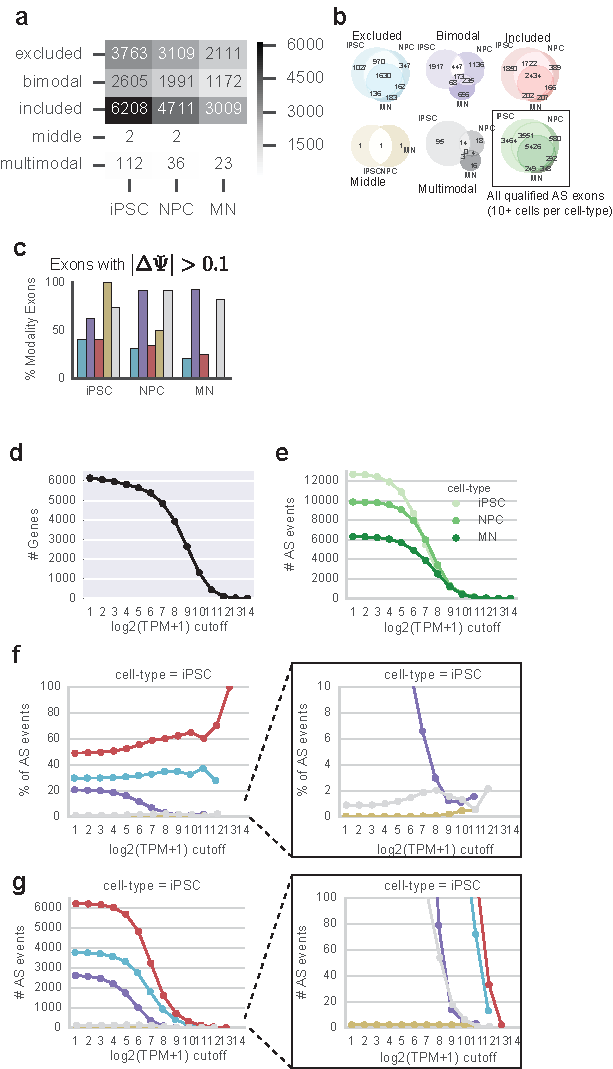
\includegraphics[width=5.8in]{figures/anchor_supplementary.pdf}
\end{figure}
%and, I'm not sure why, but one of the times I used this code the figure number wasn't augmented for the next figure, so check your figure numbers and if necessary uncomment the following line
%\addtocounter{figure}{1}
\clearpage
% --- END manual facingcaption for Supplementary Figure 2 from paper --- %



% --- BEGIN manual facingcaption for Supplementary Figure 3 from paper --- %
\clearpage
\thispagestyle{facingcaption}
\begin{figure}[h]
\captionsetup{labelformat=prev-page}
\caption[Molecular features of each splicing modality.]{
Molecular features of each splicing modality.\\
\textbf{a.}~Flanking intron sequence is more conserved in  bimodal modality. Shown in motor neurons,  intron conservation of bimodal events is slightly higher than excluded AS events.
\textbf{b.}~Barplot of mean placental mammal PhastCons score in introns flanking modality exons, across cell types. Bimodal exons in motor neurons  and NPCs are statistically enriched for higher conservation as compared to iPSCs (Kolmogorov-Smirnov test, Bonferroni-corrected).\\
\textbf{c.}~Significance (top) and boxplots (bottom) of the length of the alternative exons of different modalities. Constitutive exons are statistically enriched for longer exons, compared to excluded modality (Kolmogorov-Smirnov test, Bonferonni-corrected).\\
\textbf{d.}~Heatmap of the number of AS events in each modality overlapping with repetitive elements with AS exons, shown in iPSC. Excluded modality is statistically enriched for overlap ($q < 10^{-50}$, Hypergeometric test).\\
\textbf{e.}~Significance (top) and boxplots (bottom) of the $5^\prime$ splice site scores of the exon, specifically the splice donor site as measured by MaxEntScan. Bimodal and excluded exons have statistically significantly lower splice site scores than included exons (Kolmogorov-Smirnov test, Bonferonni-corrected).\\
\textbf{f.}~Significance (top) and boxplots (bottom) of the $3^\prime$ splice site scores of the exon, specifically the splice acceptor site as measured by MaxEntScan. Bimodal and excluded exons have statistically significantly lower splice site scores than included exons (Kolmogorov-Smirnov test, Bonferonni-corrected).\\
\textbf{g.}~Significance (top) and boxplots (bottom) of the mean expression level of genes ($\log_2(\mathrm{TPM}+1)$, x axis) harboring corresponding AS events in each modality. While events from all five modalities are detected across entire range of gene expression, genes containing bimodal exons are statistically enriched for lower expression (Kolmogorov-Smirnov test, Bonferonni-corrected).\\
\textbf{h.}~Significance (top) and boxplots (bottom) of the GC content of the alternative exons of different modalities. Excluded exons are statistically enriched for higher GC content, compared to included exons (Kolmogorov-Smirnov test, Bonferonni-corrected).\\
\textbf{i.}~Significance (top) and boxplots (bottom) of the number of exons per gene harboring corresponding modalities, measured by the maximum number of genes in any transcript of a gene. Genes containing excluded exons are statistically enriched for fewer exons per gene (Kolmogorov-Smirnov test, Bonferonni-corrected).\\
\textbf{j.}~Overview of defining ``Intron groups'' defined by cell-type, modality, and intron context, and process for obtaining their conserved $k$-mer $Z$-scores.\\
\textbf{k.}~Boxplots of the $Z$-scores of $k$-mer enrichment in the different intron groups, labeled with a colorbar of modality, intron context, and cell-type.\\
\textbf{l.}~PCA on $k$-mer $Z$-scores, with each point as a $k$-mer and the vector components as the introns. $k$-mers with principal comoponent greater than 2.5 standard deviations away from zero were labeled with the sequence, colored by the majority nucleotide. If there was a tie for the majority nucleotide, it was assigned the color grey. An interactive version of this plot can be viewed here: \url{https://plot.ly/~OlgaBotvinnik/20/modality-k-mer-z-scores-background-phenotype/}. Multimodal is not shown because its $k$-mer enrichment has a much larger range than the other modalities and overwhelms the plot.\\
\textbf{m.}~Overview of motif enrichments calculated from intron groups using a $t$-test and their transformation into PCA for visualization.\\
\textbf{n.}~Boxplots of the $t$-statistics of motif enrichment in different intron groups, labeled with colorbars of modality, intron context, and cell-type.\\
\textbf{o.}~PCA on the $t$-statistics of the Motif enrichment, labeled with the motif ID and RPB name from CISBP v0.6. An interactive version of this plot is available at\\\url{https://plot.ly/~OlgaBotvinnik/32/cisbp-motif-t-test-enrichments-background-phenotype/}
}
\label{fig:supp_modality_features}

\end{figure}
\clearpage
\begin{figure}[h]
\ContinuedFloat
\captionsetup{labelformat=empty}
\centering
% \includegraphics[width=5.8in]{sandiego.jpg}
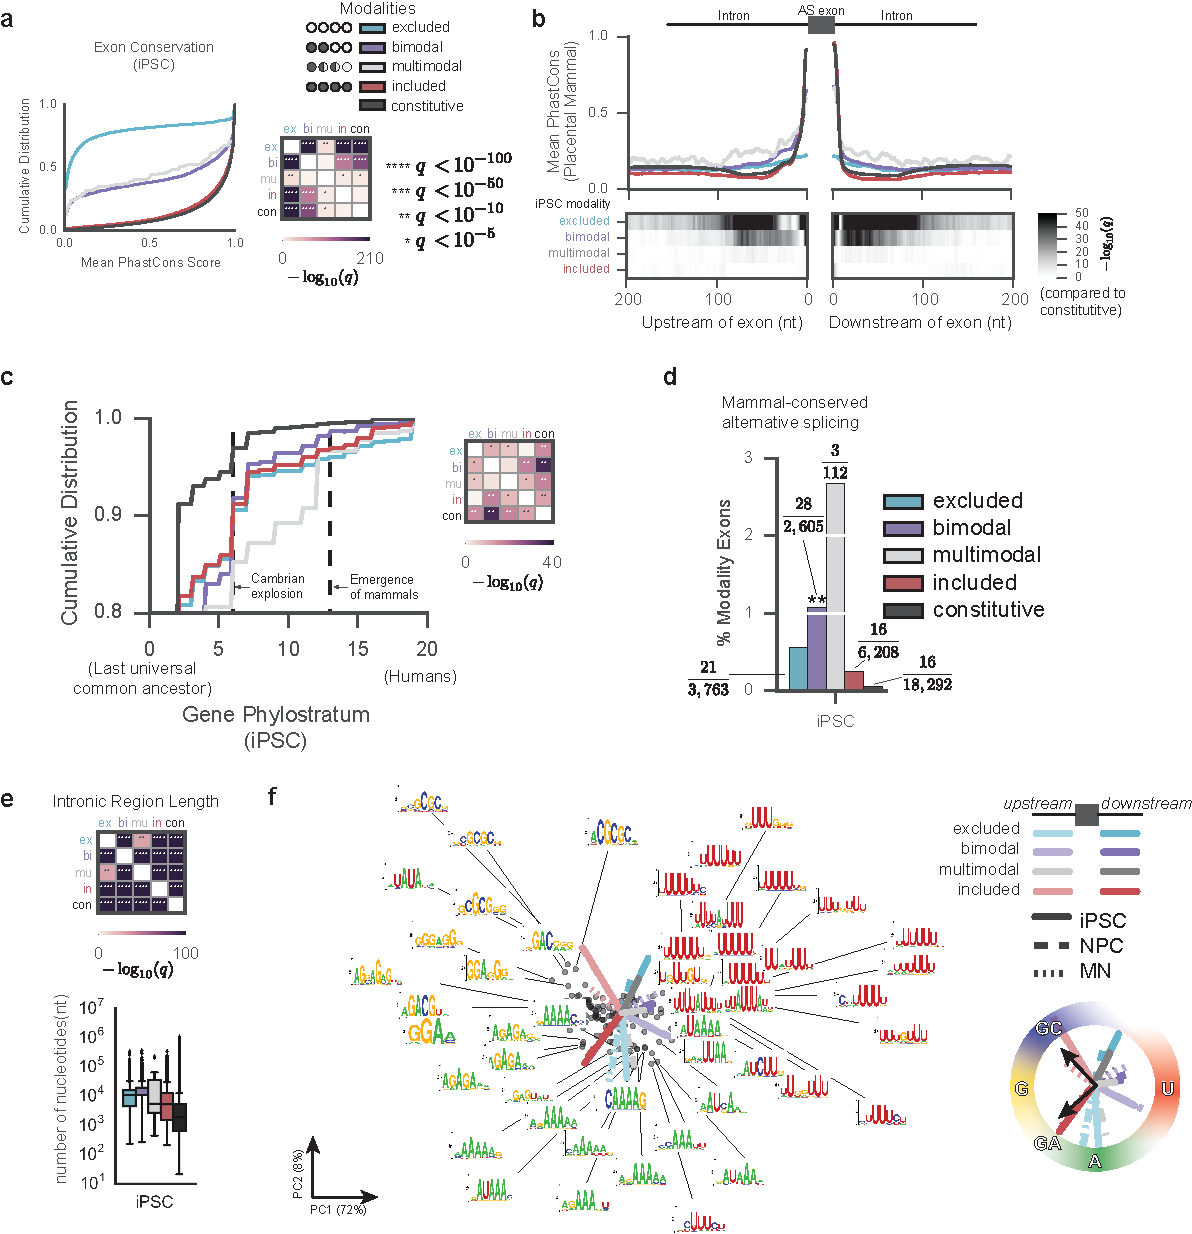
\includegraphics[width=5.8in]{figures/modality_features.pdf}
\end{figure}
%and, I'm not sure why, but one of the times I used this code the figure number wasn't augmented for the next figure, so check your figure numbers and if necessary uncomment the following line
%\addtocounter{figure}{1}
\clearpage
% --- END manual facingcaption for Supplementary Figure 3 from paper --- %



\begin{figure}[h]
  \centering
  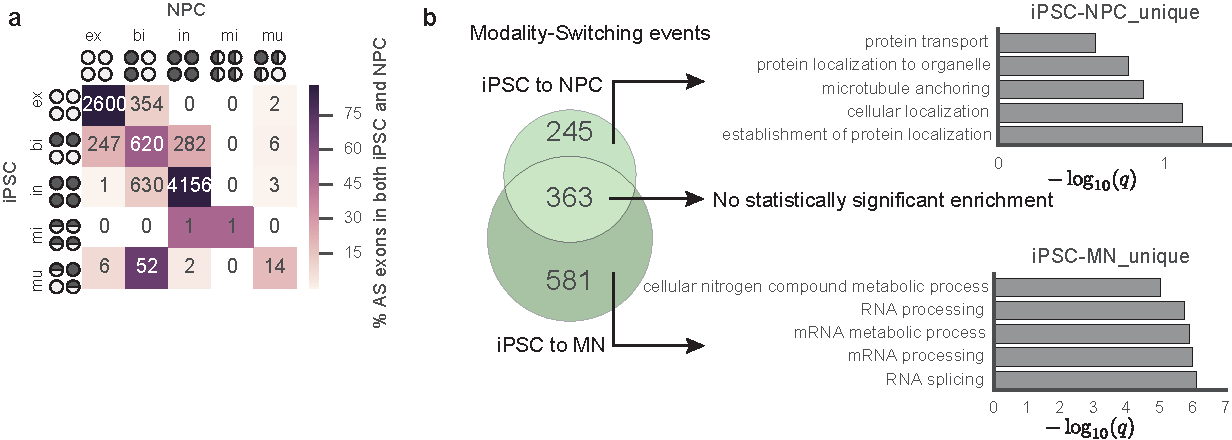
\includegraphics[width=5.8in]{figures/switching_modalities.pdf}
  \caption[Switching AS events are enriched for transcriptome and post-transcriptional regulation GO terms.]{
  Switching AS events are enriched for transcriptome and post-transcriptional regulation GO terms.\\
\textbf{a.}~AS events change modalities during iPSC to NPC transition. A total of 7,962 AS events was identified as common events in both iPSCs and MNs. Notably, $\approx 82\%$ of excluded events in iPSCs remained in excluded modality, and $\approx 84\%$ of included events in iPSCs remained as included in NPCs. In contrast 42\% of bimodal events in iPSCs switch to either included or excluded modalities in NPCs.\\
\textbf{b.}~Of the common events shared by all three populations, the events changing between iPSCs to NPCs (light green) and iPSCs to MNs (dark green). Venn diagram show the overlap between the two sets of switching AS events and GO function terms for each section of switching events.\\
}
\label{fig:switching_modalities}
\end{figure}



% --- BEGIN manual facingcaption for Supplementary Figure 5 from paper --- %
\clearpage
\thispagestyle{facingcaption}
\begin{figure}[h]
\captionsetup{labelformat=prev-page}
\caption[Highly variant AS events reveal intricacies of cell states.]{
Highly variant AS events reveal intricacies of cell states.\\
\textbf{a.}~Read coverage tracks for SNAP25 in MNs. Numbers indicate observed junction reads.\\
\textbf{b.}~Spearman correlation values of a gene's alternative splicing score ($\Psi$) to gene expression values, with a dotted line at the threshold of $R > 0.5$.\\
\textbf{c.}~Tracks from NPCs were shown to illustrate the bimodal inclusion of exon 5. Numbers indicate observed junction reads covering this SE in DYNC1I2.\\
\textbf{d-f.}~A multimodal MXE event in PKM as an example to dissect MNs into three subgroups.\\
\textbf{d.}~Genes correlating with Psi of the MXE event containing exon 9 and exon 10 (Figure 1) is able to cluster the MNs into three subgroups. Subgroup 1, mostly composed of outliers identified by $k$-means clustering (Supplementary Figure 2), contain characteristic genes for progenitors. Subgroup 2 and 3 are enriched for neuronal genes. Rows represent the genes and columns represent single cells in MNs. Genes detected in MNs and correlated with the Psi, using an emipircally-defined threshold of Spearman's $R$ greater than two standard deviations away from the mean permuted correlation values. Psi/$\Psi$ ranged from 0 (blue) to 0.5 (yellow) to 1 (red). Black and grey: cells designated as qualified cells versus outlier-cells based on $k$-means clustering. Representative genes enriched in two of the subgroups are highlighted in blue (high with exon 10 inclusion) or red (high with exon 9 inclusion). \\
\textbf{e.}~Example genes enriched in two of the subgroups of MNs. MAP2 and NRXN1 are more highly expressed in cells with $\Psi \approx 1$; ETV5 and MASTL are more highly expressed in cells with $\Psi \approx 0$. Psi scores of the MXE in PKM is plot on x-axis and $\log_2(\mathrm{TPM}+1)$ of indicated genes is plot on y-axis.\\
\textbf{f.}~Genes correlating with Psi is able to separate the three subgroups in MNs. Left, PCA using all detected genes in MNs. Right, PCA using genes correlating with Psi.\\
\textbf{g-k.} A bimodal SE event in SUGT1 as an example to dissect NPCs into two subgroups.\\
\textbf{g.}~Genes correlating with Psi of the SE event cluster the NPCs into two subgroups. Genes detected in NPCs and correlated with the Psi. Blue: cells with Psi around 0. Red: cells with Psi around 1. Light Blue to yellow: cells with Psi around 0.5. Black and grey: cells designated as qualified cells versus outlier cells based on $k$-means clustering. Representative genes enriched in two of the subgroups are highlighted in blue (high upon exon exclusion) or red (high upon exon inclusion). \\
\textbf{h.}~Expression of SUGT1 in the three populations.\\
\textbf{i.}~Psi distribution of a SE event (lower) in SUGT1 in the three populations. This event is excluded in iPSCs, and bimodal in both NPCs and MNs.\\
\textbf{j.}~Example genes enriched in the two subgroups of NPCs. TBC1D1 and ELOVL4 are more highly expressed in cells with Psi $\approx 1$; MMP16 and TSPAN14 are more highly expressed in cells with Psi ~0. Psi scores of the SE event in SUGT1 is plot on x-axis and $\log_2(\mathrm{TPM}+1)$ of indicated genes is plotted on y-axis.\\
\textbf{k.}~Only genes correlating with Psi is able to separate the two subgroups in NPCs. Left: PCA using all detected genes in NPCs. Right: PCA using genes correlating with Psi.\\
\textbf{l-o.}~PCA using all detected genes in perspective population fail to identify substructures of seemingly homogenous cells (left panel). PCA using gene correlating with each AS events (right panel) is able to identify the delicate substructures of cells.\\
\textbf{l.}~Bimodal SE event in BRD8 distinguishes iPSC substructure.\\
\textbf{m.}~Bimodal SE event in MDM4 distinguishes NPC substructure.\\
\textbf{n.}~Bimodal SE event in MEAF6 distinguishes NPC substructure.\\
\textbf{o.}~Bimodal SE event in RPN2 distinguishes MN substructure.\\
}
\label{fig:hidden_cell_states_supplementary}

\end{figure}
\clearpage
\begin{figure}[h]
\ContinuedFloat
\captionsetup{labelformat=empty}
\centering
% \includegraphics[width=5.8in]{sandiego.jpg}
\includegraphics[width=5.8in]{figures/hidden_cell_states_supplementary.pdf}
\end{figure}
%and, I'm not sure why, but one of the times I used this code the figure number wasn't augmented for the next figure, so check your figure numbers and if necessary uncomment the following line
%\addtocounter{figure}{1}
\clearpage
% --- END manual facingcaption for Supplementary Figure 5 from paper --- %


% --- BEGIN manual facingcaption for Supplementary Figure 6 from paper --- %
\clearpage
\thispagestyle{facingcaption}
\begin{figure}[h]
\captionsetup{labelformat=prev-page}
\caption[\bonvoyage on simulated datasets.]{\bonvoyage on simulated datasets.\\
\textbf{a-d.}~Datasets used for testing \bonvoyage. Uniform random noise was added in 5\% intervals to all datasets, up to 95\% noise, for 100 iterations at each noise level.\\
\textbf{a.}~Perfect middle, included, and excluded modalities, with added noise. Only 0\%, 25\%, 50\% and 75\% noise levels are shown for brevity. Top, averaged violinplots for all features at a given level of noise. Bottom, waypoint space of all features at the specified noise level.\\
\textbf{b.}~Maybe middle-included modalities, created with every combination of $0.5$ and $1.0$ values. Only the 0\% noise dataset is shown for brevity. Top, violinplots, bottom, waypoint plots.\\
\textbf{c.}~Maybe excluded-middle modalities, created with every combination of $0.0$ and $0.5$ values. Only the 0\% noise dataset is shown for brevity. Top, violinplots, bottom, waypoint plots.\\
\textbf{d.}~Maybe bimodal modalities, created with every combination of $0$ and $1$ values. Only the 0\% noise dataset is shown for brevity. Top, violinplots, bottom, waypoint plots.\\
}
\label{fig:bonvoyage_simulations}


\end{figure}
\clearpage
\begin{figure}[h]
\ContinuedFloat
\captionsetup{labelformat=empty}
\centering
% \includegraphics[width=5.8in]{sandiego.jpg}
\includegraphics[width=5.8in]{figures/hidden_cell_states_supplementary.pdf}
\end{figure}
%and, I'm not sure why, but one of the times I used this code the figure number wasn't augmented for the next figure, so check your figure numbers and if necessary uncomment the following line
%\addtocounter{figure}{1}
\clearpage
% --- END manual facingcaption for Supplementary Figure 6 from paper --- %




\begin{figure}[h]
  \centering
  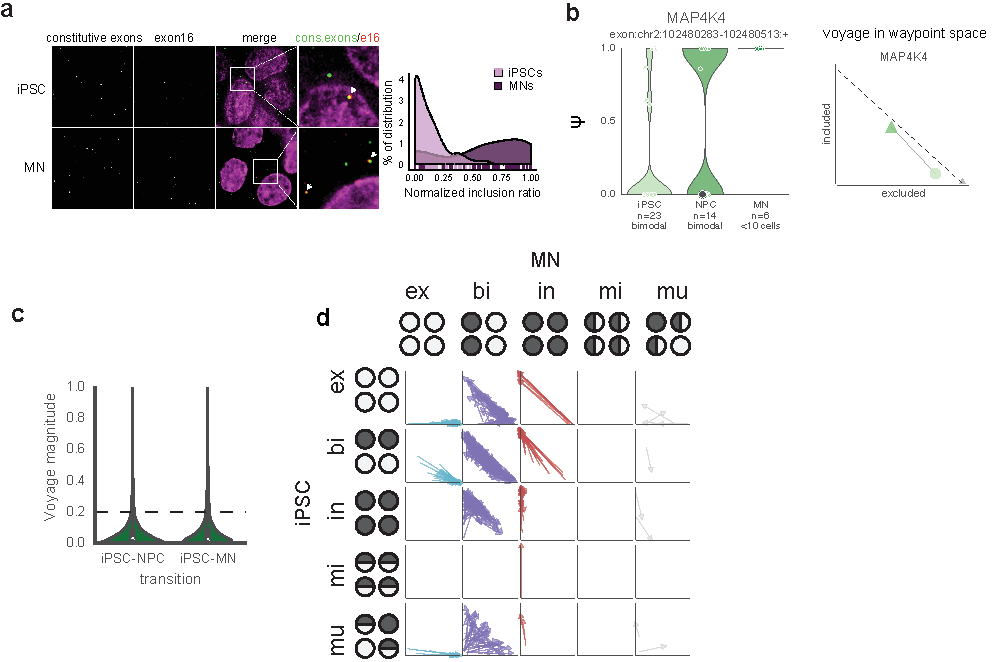
\includegraphics[width=5.8in]{figures/bonvoyage_supplementary.pdf}
  \caption[Validation of voyaging events between iPSC and MN.]{Validation of voyaging events between iPSC and MN.\\
\textbf{a.} Validation of a SE event in MAP4K4 by smRNA-FISH.\\
\textbf{b.} MAP4K4 smRNA-FISH. Left, probe sets are designed for constitutive exons and alternative exon 16. Exon 16 is excluded in iPSCs ($n = 113$, light purple with dashed line) and become more included in MNs ($n = 68$, dark purple with solid outline. Middle, quantitation of normalized inclusion of exon 16. Arrows point out foci overlapped for both constitutive and exon 16 probes. Normalized inclusion ratio is calculated by percentage of e16 probes co-localized with constitutive probes/constitutive probes, and resulting percentage is normalized by 95 percentage of the maximal percentage.\\
\textbf{c.} MAP4K4 single-cell RNA-Seq. Left, violinplots percent spliced-in inclusion values, and right, waypoint space of exon 16.\\
\textbf{d.} Magnitude of change in waypoint space (voyages) from iPSC to NPC, and iPSC to MN, with a cutoff shown as a black dashed line at 0.2.\\
\textbf{e.} Global splicing dynamics between iPSC and MN modalities, visualized as vectors from iPSC to MN  in waypoint space. Underlying data is the same as \textbf{Figure~\ref{fig:dynamic_modalities}a}. Color of arrows are coded based on event modalities in MNs.
}
\end{figure}


% --- BEGIN manual facingcaption for qPCR Validation figure --- %
\clearpage
\thispagestyle{facingcaption}
\begin{figure}[h]
  \caption[Validation of alternative splicing events by sc-qPCR.]{
  Validation of alternative splicing events by sc-qPCR.\\
\textbf{a-g.} Distribution of alternative exon inclusion by single-cell RNA-Seq for indicated events in EWSR1~(\textbf{a}), DYNC1I2~(\textbf{b}), CLTC/CLCT2~(\textbf{c}), EIF5~(\textbf{d}), THYN1~(\textbf{e}), RBPJ~(\textbf{f}), and EIF4A2~(\textbf{g}), shown in violin plots (left) and in waypoint plots (right). Percent spliced-in (Psi/$\Psi$) is calculated based on single cell RNA-seq data, illustrated in green. Black dots indicate bulk samples (~1,000 cells) for each cell type.\\
\textbf{h-n.} Distribution of percentage of inclusion by single-cell qPCR of indicated events EWSR1~(\textbf{h}), DYNC1I2~(\textbf{i}), CLTC/CLCT2~(\textbf{j}), EIF5~(\textbf{k}), THYN1~(\textbf{l}), RBPJ~(\textbf{m}), and EIF4A2~(\textbf{n}), based on single cell qPCR shown in violin plot (left) and waypoint plot (right), illustrated in blue.
}
\label{fig:validation}
\end{figure}
\clearpage
\begin{figure}[h]
\ContinuedFloat
\captionsetup{labelformat=empty}
\centering
% \includegraphics[width=5.8in]{sandiego.jpg}
\includegraphics[width=5.8in]{figures/validation_summary.pdf}
\end{figure}
%and, I'm not sure why, but one of the times I used this code the figure number wasn't augmented for the next figure, so check your figure numbers and if necessary uncomment the following line
%\addtocounter{figure}{1}
\clearpage
% --- END manual facingcaption for qPCR Validation --- %



\section{Discussion}
We developed the Expedition software suite to address key aspects of AS analysis from single-cell RNA-seq data. The Expedition suite consists of three packages that integrate the detection and quantification of AS events (outrigger) with the assignment of modalities (anchor), and a method for visualization of changes in modality (bonvoyage). As an application, Expedition was used to analyze AS in single cells from three homogenous cell-types, specifically human pluripotent stem cells, neural progenitors and motor neurons.

Many studies have performed RNA sequencing from bulk samples to measure AS, where the “relative” inclusion ($\Delta\Psi$) of alternative exons in a comparison (e.g. treatment versus control or between tissues) is the primary metric used. However, $\Delta\Psi$ comparison across all single cells are impractical. Thus, robust estimation of Psi is required to assess the distribution of Psi amongst a population of single cells. It is also important that Psi values reflect the actual biological phenomenon, such that a Psi value of 0.5 indicates that 50\% of transcripts include the alternative exon while the other 50\% exclude it. Thus, using Psi of 0.5 as a prior in probabilistic models and assessing the confidence of estimates by resampling data \cite{Katz:2010iv} is not appropriate in single cell splicing analysis as it does not eliminate cases where the observed data and annotation are incompatible (examples shown in Supplementary Software Fig. 1). In contrast, outrigger identifies splicing events by constructing de novo splicing annotation based on only junction-spanning reads, reconstructs the exon trio (quartet) for SE (MXE) events using graph traversal, and quantifies Psi. Outrigger also applies user-defined rules that ensure compatibility and sufficient read coverage of the AS events.

Anchor enables the robust classification of AS exons into five modalities (included, middle, excluded, bimodal and multimodal). Anchor characterizes AS events by their distribution and variation at the population level using a Bayesian approach, instead of estimating the noise or cell-to-cell variation of AS events (Marinov et al., 2014).  The representation of modalities in all three cell-types is remarkably consistent: ~30\% excluded, ~50\% included and ~20\% bimodal modalities, with small contributions from middle and multimodal modalities, indicating that AS is largely unimodal at the single-cell level. The ability to categorize AS distribution and variation into modalities allowed us to identify distinct sequence and evolutionary features for the three major modalities (summarized in Figure 7g). While high variance bimodal and multimodal AS events exhibit some features intermediate between included and excluded modalities, other features suggest that these AS events reflect an evolutionarily important class of exons distinct from included and excluded. High variance events contain more highly conserved and longer flanking intronic sequences. The conserved flanking intronic sequences contain cis-motifs enriched for U or UA nucleotides, in contrast to the G rich sequence in included modality. G-rich sequences have been shown to create G-quadruplexes that increase efficiency of splicing (Marcel et al., 2011; Ribeiro et al., 2015; Zizza et al., 2016), and thus the lack of G-rich sequences in bimodal may promote their flexibility to be regulated by trans-factors. Interestingly, high variance AS events are also enriched for genes present in more recently evolved phylostrata. This enrichment is concomitant with a peak of gene emergence associated with the evolution of multicellularity, shortly before the Cambrian explosion (Domazet-Loso and Tautz, 2008). At the same time, orthologous exons of the human bimodal AS events detected in our cells are also more frequently regulated as AS across other mammalian lineages (Merkin et al., 2012).

Lastly, a distinct property of multimodal AS exons is their preference to maintain protein translatability, possibly with a different function, between the two isoforms. It appears that multimodal exons provide cells flexibility to increase protein diversity without severely compromising protein-coding capacity. This is in contrast to the exons within the included or excluded modalities that tend to create or disrupt reading frames. While it is currently unknown whether these multimodal AS events are a consequence of selective allelic expression or splicing, our evidence suggests that the creation and preservation of bimodal AS exons is required to build a flexible repertoire of protein variants to efficiently cope with evolutionary or environmental changes. Moreover, we illustrate that high variance AS events reveals cellular states invisible to gene expression analysis alone, emphasizing the need to analyze AS at the single cell level. Our findings in single cells that high variance AS events are primary determinants of cell-type-specific splicing is reminiscent of findings that the cell-type- or state-specific master regulators are more likely to be variable in either gene expression (Shalek et al., 2013; Shalek et al., 2014) or epigenetic control (Buenrostro et al., 2015).
In summary, our study provides a technological framework to deconvolute the complexity of AS at a single cell level. Prospectively, Expedition can be applied to other increasingly popular data types represented by distributions of continuous variables (including but not limited to RNA-editing, nucleotide modifications such as psuedo-uridine and N6-methyl adenosine, alternative polyadenylation sites, and polyA tail lengths), providing advanced analysis to categorize, and describe these molecular features at single-cell resolution.

\section{Acknowledgements}
The authors would like to thank members of the Yeo lab for critical reading of the manuscript.  This work was supported by grants from the National Institute of Health (HG004659, NS075449, AI095277, MH107369 and HD085902), the California Institute of Regenerative Medicine (RB3-05009, RB4-06045) and the Brain Research Foundation (BRFSG-2014-14) to G.W.Y. G.W.Y. is an Alfred P. Sloan Research Fellow. O.B.B is a National Defense Science and Engineering Graduate Fellow and a NumFOCUS John Hunter Technology Fellow. We thank Jennifer Santini for technical support from Microscopy Core in the School of Medicine at UC San Diego (NS047101).
